\chapter{方法图与实验流程图}

肿瘤免疫学方向的博士后小陈正在撰写一篇小鼠肺部炎症模型的单细胞转录组论文。论文的第一张图（Figure 1A）需要放一张实验与数据分析流程图，向熟悉分子生物学但未必跑过单细胞管线的同行交代清楚：对照与处理两组小鼠的肺组织怎样一步步变成最终注释好的细胞图谱。

小陈打开图像生成工具，输入了一句英文提示词（意为“创建一张专业、色彩丰富的单细胞 RNA 测序实验与数据分析流程图，从组织到细胞类型注释，横向 16:9”）：

\begin{Prompt}
Create a professional, colorful flowchart of a single-cell RNA sequencing experiment and
data analysis workflow, from tissue to cell type annotation. Landscape 16:9.
\end{Prompt}

不到一分钟，屏幕跳出了一张十一格彩色信息图（图~\ref{fig:ch06-01}）。画面上方挂着深蓝色总标题，湿实验和生物信息学分析分别配了醒目的渐变色横幅，培养管、微流控通道、测序仪、小提琴图和散点图一应俱全。

\begin{figure}[htbp]\centering
\begin{tikzpicture}
\definecolor{ChSixBad}{HTML}{C0392B}
\node[anchor=south west,inner sep=0] (img) at (0,0) {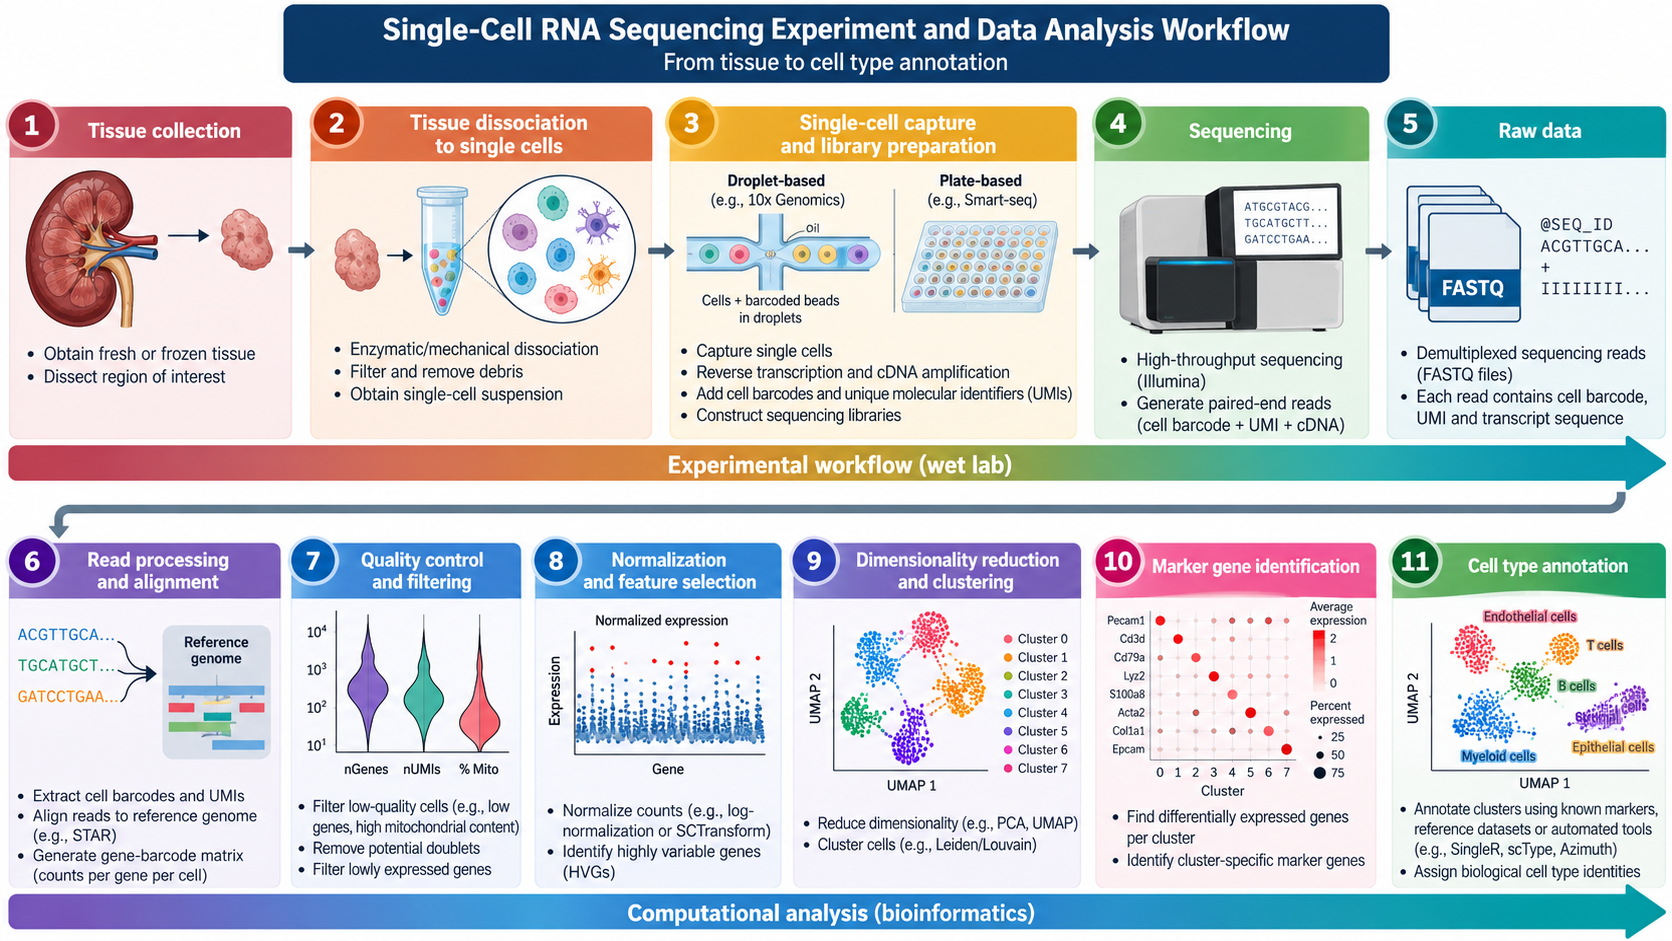
\includegraphics[width=\linewidth]{figures/ch06/ch06-01-v1-vague.png}};
\begin{scope}[x={(img.south east)},y={(img.north west)}]
  \tikzset{badmark/.style={draw=white,line width=0.8pt,fill=ChSixBad,text=white,circle,font=\sffamily\bfseries\scriptsize,inner sep=1.1pt,minimum size=4.2mm}}
  \node[badmark] at (0.09,0.74) {1};
  \node[badmark] at (0.36,0.80) {2};
  \node[badmark] at (0.91,0.78) {3};
  \node[badmark] at (0.24,0.36) {4};
  \node[badmark] at (0.55,0.36) {5};
  \node[badmark] at (0.91,0.28) {6};
\end{scope}
\end{tikzpicture}
\caption{只用一句话提示词生成的单细胞测序流程图初稿（教学用失败示例）。编号指出的问题：（1）左上画成单个肾脏，未体现对照与处理两份肺组织样本的并行处理；（2）湿实验缺少细胞活率与文库两道质控门，第 3 格同时塞入液滴法与孔板法并略去文库混合点；（3）第 5 格把数据产物 FASTQ 画成与测序同级的操作步骤；（4）第 7 格质控画成普通串联面板，没有通过与不通过两个出口；（5）第 9 格把降维、近邻图、聚类与 UMAP 笼统合为一格，看不出近邻图向聚类与可视化的分叉；（6）终点缺少异常簇返回复核的反馈回路，右下角“Stromal cells”标签直接压在紫色散点上，且全图文字锁死在位图中无法编辑。}\label{fig:ch06-01}
\end{figure}

然而把这张初稿放大到 200\% 逐格检查时，六处硬伤接连暴露（图~\ref{fig:ch06-01} 红圈 1–6）：左上角第 1 格画了一颗肾脏而非肺组织（因为提示词只写了泛泛的“tissue”），且全图只画了一条单样本路径，看不出对照组与处理组两个样本在哪里独立处理、在哪里混合测序；第 3 格把液滴法（10x Genomics）和孔板法（Smart-seq）两种实验路线并排塞进同一个步骤框，还将单细胞捕获、逆转录、cDNA 扩增与文库构建全部压成一个黑箱，中间既无细胞计数活率质控，也无文库片段质控；第 5 格把数据产物“Raw data（FASTQ）”画成了与“测序”同级的操作步骤框；下排第 7 格虽有小提琴图表示质控过滤，却只是普通串联面板，没有“合格放行、不合格排查”的出口；第 9 格把降维与聚类合画成一张带虚线圆圈的 UMAP 图，掩盖了“在主成分空间构建近邻图，再分别分叉去做聚类和 UMAP 展示”的分析拓扑；第 11 格注释终点不仅缺少发现低质量簇时退回上游的反馈路径，右下角“Stromal cells”字样还直接压在紫色细胞簇上，且高光阴影、渐变色带与大段说明文字全部锁死在位图里，缩排到期刊尺寸后既笨重又无法修改。

审稿人只需看五秒钟，就会发现图面与方法文字处处矛盾；小陈却在对话框里追着模型改了一下午，修好了器官图标，分支和箭头又乱了套。本章的办法是：\textbf{先把步骤写成表，再用确定性工具画结构骨架，最后才让 AI 负责图标与视觉风格。}

\section{流程图回答什么问题}

在科研论文里，方法图与实验流程图（workflow diagram）承担的任务和第 7 章要讨论的机制图截然不同。机制图回答的是“为什么会发生”——分子、细胞或组件之间通过什么因果作用产生效应；流程图回答的则是\textbf{“研究工作是怎么一步步做下来的”}——实验与计算包含哪些操作步骤，每一步接收什么输入、交出什么产物，在什么参数或质控条件下放行或退回，以及多份样本或多条计算支路在哪里分叉、在哪里汇合。

具体而言，一张结构清晰的流程图必须向读者交代清楚四个基本要素：
\begin{enumerate}
\item \textbf{步骤（做什么）：}对实验材料或数据集施加的具体操作，例如“组织解离”“文库构建”“比对与 UMI 计数”或“Leiden 聚类”。图中的每一个步骤框对应的都应当是一个明确的动作，而不是笼统的学科名词。
\item \textbf{产物（得到什么、交接什么）：}上一步操作结束时产生、并作为下一步输入的实体材料或数据对象，例如“单细胞悬液”“带条形码的 cDNA”“FASTQ 文件”或“过滤后计数矩阵”。在关键形态转换处把产物单独标出，读者才能看懂上下游步骤之间到底传递了什么。
\item \textbf{条件与质控（何时放行、何时返回）：}决定流程能否继续往下推进的实验参数与质量判断节点。凡是标为“质控”或“检查”的节点，在逻辑上都必然存在两种去向：合格时沿主干放行到下一步，不合格时沿反馈路径退回上游步骤重新优化、补样或调整过滤条件。
\item \textbf{分支与合并（谁和谁并行、在哪里汇合）：}真实的实验与计算流程很少是一根到底的直线。对照与处理样本往往先各自独立解离、捕获、建库，到上机测序前才按比例混合；计算分析中，主成分空间的近邻图既要送去运行图聚类算法以划分细胞亚群，又要送去计算二维嵌入坐标用于散点图展示。分叉点与合并点的位置直接反映了实验设计与分析逻辑。
\end{enumerate}

厘清这四个要素后，必须划定一条核心边界：\textbf{流程箭头只表示时间先后与物料或数据交接，不表示生物学因果、作用机制或效应大小。}例如在单细胞制备流程中，“组织解离 $\rightarrow$ 单细胞悬液”是一条标准的流程关系，表示前一步操作产出了后一件实验材料；但前人研究指出，较长时间的温热酶解离可能诱导部分组织亚群出现早期应激相关基因表达升高（van den Brink 等，2017）。后一句话属于实验操作引发的生物学效应或质控伪影提醒，如果用同一根实心流程箭头画成“组织解离 $\rightarrow$ 应激基因表达升高”，就会把实验操作步骤与细胞内在转录响应混为一谈。正确的处理方式是用浅灰色虚线引线把这类机制或质控背景写成旁注，或者直接交代在图注里。

为了防止读者在读图时靠猜来区分步骤、产物和判断条件，本书采用一套固定的流程图节点与箭头语法（图~\ref{fig:ch06-02}）。

\begin{figure}[htbp]\centering
% FIG ch06-02 flow grammar (Chinese)%
% Shared styles for chapter 6 workflow TikZ figures.%
% Every figure inputs this file, so commands are defined with \providecommand.%
\providecolor{BookTeal}{HTML}{176C68}%
\providecolor{BookInk}{HTML}{23363E}%
\providecolor{BookRule}{HTML}{C8D6D6}%
\providecolor{BookPale}{HTML}{F1F6F5}%
\definecolor{WetPale}{HTML}{FBF1EA}%
\definecolor{Wet}{HTML}{B5653A}%
\definecolor{Seq}{HTML}{8A6D1F}%
\definecolor{DryPale}{HTML}{EEF4F7}%
\definecolor{Dry}{HTML}{2F6F8F}%
\definecolor{ChSixFeedback}{HTML}{7A8A90}%
\definecolor{ChSixBad}{HTML}{C0392B}%
\usetikzlibrary{arrows.meta,positioning,shapes.geometric,shapes.misc,fit,backgrounds,calc}%
\ifdefined\ChSixLayersReady\else%
  \pgfdeclarelayer{chsixlane}%
  \pgfsetlayers{chsixlane,background,main}%
  \def\ChSixLayersReady{}%
\fi%

\tikzset{%
  chsix/.style={font=\sffamily\scriptsize, text=BookInk, align=center},%
  flowstep/.style={%
    chsix, rounded corners=2pt, draw=Wet, line width=0.45pt, fill=white,%
    text width=19mm, minimum height=7.4mm, inner sep=1.3pt,%
  },%
  flowstepdry/.style={flowstep, draw=Dry},%
  flowstepseq/.style={flowstep, draw=Seq},%
  artifact/.style={%
    chsix, trapezium, trapezium left angle=70, trapezium right angle=110,%
    trapezium stretches=true,%
    draw=BookInk, line width=0.45pt, fill=white,%
    minimum height=6.2mm, inner sep=1.2pt,%
  },%
  gate/.style={%
    chsix, diamond, aspect=1.7, draw=BookInk, line width=0.45pt, fill=white,%
    text width=12mm, inner sep=0.6pt, minimum height=8mm,%
  },%
  opt/.style={flowstep, dashed, draw=BookInk!70},%
  optdry/.style={flowstepdry, dashed, draw=BookInk!70},%
  stack/.style={flowstep},%
  link/.style={-{Stealth[length=1.6mm]}, semithick, draw=BookInk},%
  linkthin/.style={-{Stealth[length=1.2mm]}, thin, draw=BookInk!80},%
  back/.style={-{Stealth[length=1.5mm]}, dashed, draw=ChSixFeedback},%
  conn/.style={%
    circle, draw=BookInk, line width=0.5pt, minimum size=4.6mm,%
    font=\sffamily\scriptsize\bfseries, inner sep=0pt, text=BookInk,%
  },%
  lanetitle/.style={font=\sffamily\bfseries\small, text=BookInk, align=left},%
  passlabel/.style={font=\sffamily\scriptsize, text=BookInk, fill=white, inner sep=0.7pt, align=center},%
  mergelabel/.style={font=\sffamily\scriptsize, text=BookInk, fill=white, inner sep=0.8pt, align=center},%
  taglab/.style={font=\sffamily\scriptsize, text=ChSixFeedback, fill=white, inner sep=0.8pt, align=center},%
  gramcap/.style={font=\sffamily\scriptsize, text=BookInk, align=left, anchor=west},%
}%

% Offset card behind a two-sample step. Text stays on the front node only.%
\providecommand{\ChSixCardBack}[1]{%
  \begin{pgfonlayer}{background}%
    \draw[Wet, line width=0.45pt, rounded corners=2pt, fill=white]%
      ([shift={(-0.55mm,0.55mm)}]#1.south west)%
      rectangle ([shift={(-0.55mm,0.55mm)}]#1.north east);%
  \end{pgfonlayer}%
}%
% #1 options, #2 name, #3 position (with parentheses), #4 text%
\providecommand{\ChSixCard}[4]{%
  \node[stack, #1] (#2) at #3 {#4};%
  \ChSixCardBack{#2}%
}%

\providecommand{\ChSixMaybeLabel}[1]{%
  \ifdefined\nolabels\else#1\fi%
}%

\providecommand{\ChSixIcon}[2]{%
  \ifdefined\ChSixShowIcons%
    \IfFileExists{#1}{%
      \node[anchor=south, inner sep=0] at ([yshift=0.7mm]#2.north)%
        {\includegraphics[height=5.4mm]{#1}};%
    }{}%
  \fi%
}%
%
\begin{tikzpicture}[x=1mm, y=1mm, font=\sffamily\scriptsize, text=BookInk]%
  \node[anchor=north west, font=\sffamily\bfseries\small] (titleL) at (0,0) {节点与箭头语法};%
  \draw[BookRule, line width=0.4pt] (0,-7) rectangle (128,-126);%

  \node[flowstep] (g1) at (16,-14) {操作步骤};%
  \node[gramcap] at (36,-14) {圆角矩形——做什么};%

  \node[artifact] (g2) at (16,-25) {产物};%
  \node[gramcap] at (36,-25) {平行四边形——得到什么、交给下一步什么};%

  \node[gate] (g3) at (16,-38) {质控};%
  \node[passlabel, anchor=west] at ([xshift=1.5mm]g3.east) {通过};%
  \node[taglab, anchor=north west] at ([xshift=1.5mm, yshift=-0.6mm]g3.south east) {不通过};%
  \node[gramcap] at (36,-38) {菱形——须有两个出口（通过 / 不通过）};%

  \node[opt] (g4) at (16,-50) {可选步骤};%
  \node[gramcap] at (36,-50) {虚线圆角矩形};%

  \node[stack] (gs1) at (13,-61) {};%
  \ChSixCardBack{gs1}%
  \node[stack] (gs2) at (16.2,-61) {每样本};%
  \node[gramcap] at (36,-61) {错位叠放——每个样本分别进行};%

  \draw[link] (6,-72) -- ++(16,0);%
  \node[gramcap] at (36,-72) {实线箭头——顺序与交接};%

  \draw[back] (6,-83) to[out=20, in=160] (24,-83);%
  \node[gramcap] at (36,-83) {虚线弧——反馈或返回};%

  \fill (16,-94) circle (0.7pt);%
  \node[gramcap] at (36,-94) {实心圆点——分叉 / 合并点};%

  \node[conn] (gc) at (16,-105) {A};%
  \node[gramcap] at (36,-105) {圆形连接符——跨行续接};%

  \fill[WetPale, draw=Wet, line width=0.3pt] (6,-116) rectangle (16,-122);%
  \fill[DryPale, draw=Dry, line width=0.3pt] (18,-116) rectangle (28,-122);%
  \node[gramcap] at (36,-119) {泳道底色——湿实验 / 计算};%

  \node[anchor=north west, font=\sffamily\bfseries\small] (titleR) at (0,-130) {流程箭头 ≠ 因果};%
  \node[flowstep] (d1) at (18,-144) {组织解离};%
  \node[artifact] (d2) at (46,-144) {单细胞悬液};%
  \draw[link] (d1) -- (d2);%
  \node[gramcap] at (68,-144) {流程：先后与交接};%

  \node[flowstep] (e1) at (18,-160) {组织解离};%
  \node[gramcap] at (40,-160) {$\Rightarrow$ 应激相关基因表达升高};%
  \draw[BookInk!45, densely dotted] (e1.east) -- ++(6,0);%
  \node[gramcap, anchor=north west, text width=120mm] at (0,-170)%
    {机制或因果信息写成注释或图注，不画成流程箭头（van den Brink 等 2017）。};%
\end{tikzpicture}%

\caption{本书流程图使用的节点与箭头。每种形状只表示一种含义。下框：流程箭头表示先后与交接；解离可能诱导应激相关基因表达（van den Brink 等，2017）这类机制信息写成注释，不画成流程箭头。}\label{fig:ch06-02}
\end{figure}

如图~\ref{fig:ch06-02} 所示，这套语法遵循“一形一义”的视觉编码原则（Wong，2010；Wong，2011a）：
\begin{itemize}
\item \textbf{圆角矩形表示操作步骤：}框内写动宾短语或操作名称（如“组织解离”“PCA 降维”），不混写输入输出文件名。
\item \textbf{平行四边形表示数据或材料产物：}放在关键交接步骤之间或分支终点，标明交付的实物或数据结构（如“单细胞悬液”“原始计数矩阵”）。
\item \textbf{菱形表示质控或条件判断：}每一个菱形节点都必须同时画出“通过”和“不通过”两个出口。
\item \textbf{虚线圆角矩形表示可选步骤：}用于标记随具体组织类型、实验设计或软件路线而异的操作（如“红细胞裂解”“批次整合”）。
\item \textbf{错位叠放的双层圆角矩形表示多样本分别进行：}当对照组与处理组样本按完全相同的规程各自独立完成某一步时，用两张轻微错位叠放的卡片表示“每个样本分别进行”，既省去重复画两条平行长链的版面开销，又比单层方框多传递了样本独立性信息。
\item \textbf{实线箭头与虚线弧区分顺向交接与反馈迭代：}深灰实线配实心三角箭头专用于顺向交接；中灰虚线弧专用于质控未通过或下游结果异常时向上游步骤的返回与迭代。
\item \textbf{实心圆点、圆形连接符与泳道色带组织宏观版面：}分叉与合并处点一枚实心小圆点；跨行或跨泳道续接时使用写有同一字母的圆形连接符（如“A”）；全图背景按阶段铺设浅暖色（湿实验与测序）与浅冷色（计算分析）两条水平泳道色带，并在左上角配粗体泳道标题，确保即使灰度打印也能一眼分清实验台操作与计算机分析。
\end{itemize}

\section{从方法记录到步骤表}

为什么把论文方法部分的文字直接贴给 AI，往往画不出合格的流程图？因为论文方法章节是按\textbf{文字叙述顺序}组织的，而流程图必须按\textbf{输入与产物的交接关系}组织。

在文字段落里，作者常把同类概念合在一起写，或者用“随后”“同时”“必要时”一笔带过分支条件；可是一旦落到图纸上，每一个框连向哪里、两条线在哪个节点汇合，都必须有唯一确定的答案。因此，从方法记录走向流程图的第一步，不是构思配色和图标，而是把叙述文字拆解成一张结构化的\textbf{步骤表}。

下面以本章主案例——比较对照与处理两种条件下小鼠肺组织细胞组成的微滴法 3$'$ 端单细胞 RNA 测序流程——演示这一转换过程。本案例的实验与分析步骤依据单细胞测序领域的通用规程与综述整理：液滴捕获、细胞条形码（cell barcode）与唯一分子标识符（UMI）原理参照 Islam 等（2014）、Macosko 等（2015）、Zheng 等（2017）及 Hwang 等（2018）；计算质控、标准化、高变基因选择、降维、近邻图、聚类与细胞类型注释流程参照 Wolf 等（2018）、Luecken 与 Theis（2019）及 Heumos 等（2023）；Leiden 聚类算法参照 Traag 等（2019）；双细胞检测与环境游离 RNA 校正分别参照 Wolock 等（2019）与 Young 和 Behjati（2020）。

需要明说的是，下面这段材料是本书编写的\textbf{教学用方法记录}，按上述通用流程组织，不对应任何具体论文的真实测量，因此凡涉及酶浓度、消化时间、活率阈值或过滤阈值的参数，一律写成“〔作者填写〕”：

\begin{BookNote}
对照与处理组小鼠各取肺组织一份，分别处理。组织剪碎后在〔酶与浓度〕中于〔温度〕消化〔时间〕，期间机械吹打；经〔孔径〕细胞筛过滤，〔可选：红细胞裂解；死细胞去除〕。用〔方法〕计数并评估活率，活率低于〔阈值〕时重新优化解离。合格的单细胞悬液按〔目标细胞数〕上样到微流控芯片，细胞与带条形码的凝胶珠共同包裹在油包水微滴中；微滴内细胞裂解，mRNA 经含细胞条形码、UMI 与 poly(dT) 的引物逆转录。破乳后纯化并扩增 cDNA，检测片段分布。cDNA 经片段化、末端修复与加 A、接头连接和样本索引 PCR 构建文库，检测文库片段大小与浓度后，两个样本的文库按〔比例〕混合，在〔测序平台〕上双端测序（Read 1：细胞条形码 + UMI；Read 2：cDNA 片段）。

测序数据拆分为 FASTQ 后，比对到〔参考基因组版本〕并按 UMI 计数，得到每个样本的基因 $\times$ 条形码矩阵；识别含细胞的条形码，按 UMI 总数、检测基因数和线粒体基因读段比例过滤低质量细胞（阈值〔作者依分布确定〕），同时进行双细胞检测与环境 RNA 校正（可选）。两样本合并后进行文库大小标准化与对数转换，选择高变基因，PCA 降维（如有批次效应则整合），构建 $k$ 近邻图，在图上用 Leiden 算法聚类，并计算 UMAP 用于可视化。对每个簇找标志基因，结合已知标志物与参考数据集注释细胞类型；若出现低质量簇或分辨率不当，返回调整质控阈值或聚类分辨率。
\end{BookNote}

我们可以先让对话式 AI 从这段方法文字中抽出候选步骤行、提示可能遗漏的中间产物与质控口，但作者必须紧握两条主审原则：第一，\textbf{AI 不得编造任何实验参数或质控阈值}。大语言模型在整理方法表时，极易顺手补出看起来合理的温度、消化时长、活率百分比或线粒体比例阈值——这些数字必须全部标为“待确认”，由作者对照原始实验本与分析脚本亲自填写。第二，\textbf{每一步占一行，明确写出步骤编号、泳道、输入、产物、关键条件、质控出口与下游编号}。整理核实后的步骤表见表~\ref{tab:ch06-01}，它是本章绘图与核验的“唯一事实来源”。

\begin{table}[htbp]\centering\scriptsize
\setlength{\tabcolsep}{2pt}
\renewcommand{\arraystretch}{1.08}
\caption{液滴法单细胞 RNA 测序实验与分析流程步骤表（绘图的唯一事实来源）。}\label{tab:ch06-01}
\begin{tabularx}{\linewidth}{@{}l>{\raggedright\arraybackslash}p{15mm}l>{\raggedright\arraybackslash}p{16mm}>{\raggedright\arraybackslash}p{16mm}YYl@{}}
\toprule
\textbf{ID} & \textbf{步骤} & \textbf{泳道} & \textbf{输入} & \textbf{产物} & \textbf{关键条件（作者填写）} & \textbf{质控/判断与可选分支} & \textbf{下游} \\
\midrule
W1 & 组织采集 & 湿实验 & 小鼠（对照、处理） & 新鲜肺组织 & 采样时间、保存方式 & 两样本分别进行 & W2 \\
W2 & 组织解离 & 湿实验 & 肺组织 & 细胞悬液（粗） & 酶、浓度、温度、时间、机械方式 & 两样本分别进行 & W3 \\
W3 & 过滤与清洗 & 湿实验 & 粗悬液 & 单细胞悬液 & 筛孔径 & 可选 W3a 红细胞裂解、W3b 死细胞去除（虚线框） & Q1 \\
Q1 & 细胞计数与活率 & 湿实验 & 单细胞悬液 & 计数、活率记录 & 计数方法、活率阈值 & 通过 $\rightarrow$ W4；不通过 $\rightarrow$ 返回 W2（反馈弧） & W4 \\
W4 & 微滴捕获与条形码标记 & 湿实验 & 单细胞悬液、凝胶珠、油 & 微滴（每滴$\approx$一细胞一珠） & 目标细胞数、芯片类型 & 两样本分别上样 & W5 \\
W5 & 微滴内逆转录；破乳；cDNA 扩增 & 湿实验 & 微滴 & 带条形码的 cDNA & 扩增循环数 & cDNA 片段分布（记录，不设分支） & W6 \\
W6 & 文库构建 & 湿实验 & cDNA & 测序文库（每样本一索引） & 片段化、接头、索引 PCR 循环数 & 两样本分别建库 & Q2 \\
Q2 & 文库质控 & 湿实验 & 测序文库 & 片段大小、浓度记录 & 方法、合格标准 & 通过 $\rightarrow$ S1；不通过 $\rightarrow$ 返回 W6 & S1 \\
S1 & 文库混合与测序 & 湿实验（测序） & \textbf{两个样本的文库}（合并点） & 原始读段 $\rightarrow$ FASTQ & 平台、读长、测序深度 & 经连接符 A 交接至计算泳道 & C1 \\
C1 & 比对与 UMI 计数 & 计算 & FASTQ、参考基因组与注释 & 原始计数矩阵（每样本） & 软件与版本、参考版本 & 按样本分别比对计数 & C2 \\
C2 & 细胞识别 & 计算 & 原始计数矩阵 & 含细胞的条形码 & 方法 & 区分含细胞微滴与空滴 & Q3 \\
Q3 & 细胞级质控 & 计算 & 细胞矩阵 & 过滤后矩阵 & UMI 数、基因数、线粒体比例阈值 & 并行可选：C3a 双细胞检测 $\parallel$ C3b 环境 RNA 校正 & C4 \\
C4 & 合并样本；标准化与对数转换 & 计算 & \textbf{两样本过滤后矩阵}（合并点） & 标准化表达矩阵 & 方法 & 两样本矩阵在此合并 & C5 \\
C5 & 选择高变基因 & 计算 & 标准化矩阵 & 高变基因列表 & 基因数 & — & C6 \\
C6 & PCA 降维 & 计算 & 高变基因表达 & 主成分坐标 & 主成分数 & 可选 C6a 整合/批次校正（虚线框） & C7 \\
C7 & 构建 $k$ 近邻图 & 计算 & 主成分坐标 & 近邻图 & $k$ 值 & \textbf{分叉} $\rightarrow$ C8 与 C9 & C8、C9 \\
C8 & 聚类（Leiden） & 计算 & 近邻图 & 簇标签 & 分辨率 & — & C10 \\
C9 & UMAP 嵌入 & 计算 & 近邻图 & 二维坐标（\textbf{仅用于展示}） & 参数 & 终点，不连向 C8 或 C11 & （展示） \\
C10 & 标志基因分析 & 计算 & 标准化矩阵 + 簇标签 & 每簇标志基因表 & 检验方法 & — & C11 \\
C11 & 细胞类型注释 & 计算 & 标志基因表、标志物、参考集 & 注释后的细胞图谱 & 参考数据集版本 & 发现低质量簇/分辨率不当 $\rightarrow$ 返回 Q3 或 C8 & 终点 \\
\bottomrule
\end{tabularx}
\end{table}

细读表~\ref{tab:ch06-01}，它在动笔前帮作者理清了五个极易在画图时出错的方法学细节：
\begin{enumerate}
\item \textbf{两处合并点的位置不同：}湿实验中，对照与处理两个样本从 W1 到 Q2 各自独立处理，加上不同样本索引（sample index）后在 S1（文库混合与测序）处第一次合池测序；计算分析中，下机 FASTQ 按索引拆分后，仍先按样本分别比对计数（C1）、识别含细胞条形码（C2）并执行细胞级质控（Q3），直到 C4（合并与标准化）才将两个样本的过滤后矩阵合并。
\item \textbf{微滴内操作与破乳后扩增：}在 3$'$ 端液滴平台的一般流程中，微滴内部完成的是细胞裂解与 mRNA 逆转录，而 cDNA 扩增是在破乳纯化之后进行的。由于不同化学版本的具体细节略有差异，表~\ref{tab:ch06-01} 将“微滴内逆转录、破乳与 cDNA 扩增”合记为 W5，避开版本差异。
\item \textbf{理想化微滴示意与计算去噪的呼应：}W4 的图标通常画成“每滴含一个细胞与一颗凝胶珠”的理想化状态；但实际微流控上样时，为控制多细胞共包裹率，多数微滴为空滴（含环境游离 RNA），少数微滴含两个及以上细胞（双细胞）。这也正是计算泳道必须设置 C2 细胞识别、C3a 双细胞检测与 C3b 环境 RNA 校正的原因。
\item \textbf{可选步骤与整合位置：}不同分析软件中“整合/批次校正”所处的位置不同（本表放在 C6 PCA 降维之后作为虚线可选框 C6a，代表在主成分空间整合的方法；也有方法在标准化或特征选择阶段整合）；同样，C3a 双细胞检测与 C3b 环境 RNA 校正在不同管线中的先后关系不同，本表画成 Q3 下的并行可选分支，并在图注中明确声明这是教学简化。
\item \textbf{C7 处的平行分叉：}C7（$k$ 近邻图）分叉出 C8（Leiden 聚类）与 C9（UMAP 嵌入），C9 不连向 C8 或 C11。作者若确实把簇标签投射到 UMAP 图上辅助人工检查注释，可在图注中写“UMAP 用于展示与检查”，图中不画依赖箭头。
\end{enumerate}

由 AI 协助起草步骤表后，作者必须对照实验本与分析脚本逐项勾选表~\ref{tab:ch06-02} 的九项确认清单。凡是实际实验中没有做的可选步骤（如未做红细胞裂解或死细胞去除），在正式论文配图中应直接删掉虚线框，不保留“可能做过”的模糊表述。

\begin{table}[htbp]\centering\footnotesize
\setlength{\tabcolsep}{4pt}
\renewcommand{\arraystretch}{1.15}
\caption{作者确认清单（AI 起草步骤表后必须由作者逐项勾选）。}\label{tab:ch06-02}
\begin{tabularx}{\linewidth}{@{}c>{\raggedright\arraybackslash}p{28mm}Y@{}}
\toprule
\textbf{序号} & \textbf{核对维度} & \textbf{必须由作者对照原始实验记录或分析代码确认的具体事项} \\
\midrule
1 & 样本批次与通道 & 两个样本是否在同一批次、同一张芯片的不同通道处理？（决定是否画 C6a“整合”可选框） \\
2 & 湿实验可选步骤 & 是否实际做了 W3a 红细胞裂解、W3b 死细胞去除？未做就删掉虚线框，而不是保留“可能做过”。 \\
3 & 湿实验质控去向 & Q1、Q2 的合格标准和“不通过”的实际处理方式（返回优化、补样，还是终止）。 \\
4 & 测序读长结构 & 测序平台及双端读长结构（Read 1 / Read 2 各含什么序列）是否与所用试剂说明书一致。 \\
5 & 比对与参考版本 & C1 比对计数软件名称与版本、参考基因组与基因注释的具体版本。 \\
6 & 细胞质控与去噪 & Q3 的三个过滤阈值是否按数据分布确定、是否每个样本分别设定；C3a、C3b 是否真的做了。 \\
7 & 聚类空间来源 & C8 聚类所用的近邻图来自 PCA（或整合后的低维空间），而不是二维 UMAP 空间。 \\
8 & 细胞注释依据 & C11 注释依据（标志基因列表、参考数据集版本）以及是否有研究者人工复核。 \\
9 & 表图双向闭环 & 图中每个框都能在表~\ref{tab:ch06-01} 中找到对应行；表中每行都在图中出现或在图注中声明省略。 \\
\bottomrule
\end{tabularx}
\end{table}

\section{结构先行：用确定性工具画骨架}

拿到核实无误的步骤表后，为什么不直接把步骤表喂给图像生成模型出整图？

因为\textbf{图像生成模型在像素层面“画得像”，但不保证箭头数量、方向和连接对象正确}；而结构错误恰恰是流程图最致命的错误。最稳妥的做法是“结构先行”：先用确定性绘图工具（TikZ、PowerPoint、draw.io 或 Illustrator 等任何能对齐节点与连接线的工具）严格按表~\ref{tab:ch06-01} 画出\textbf{结构骨架图}（图~\ref{fig:ch06-03}）。

\begin{figure}[htbp]\centering
\resizebox{\linewidth}{!}{% FIG ch06-03 skeleton (Chinese)%
% Shared styles for chapter 6 workflow TikZ figures.%
% Every figure inputs this file, so commands are defined with \providecommand.%
\providecolor{BookTeal}{HTML}{176C68}%
\providecolor{BookInk}{HTML}{23363E}%
\providecolor{BookRule}{HTML}{C8D6D6}%
\providecolor{BookPale}{HTML}{F1F6F5}%
\definecolor{WetPale}{HTML}{FBF1EA}%
\definecolor{Wet}{HTML}{B5653A}%
\definecolor{Seq}{HTML}{8A6D1F}%
\definecolor{DryPale}{HTML}{EEF4F7}%
\definecolor{Dry}{HTML}{2F6F8F}%
\definecolor{ChSixFeedback}{HTML}{7A8A90}%
\definecolor{ChSixBad}{HTML}{C0392B}%
\usetikzlibrary{arrows.meta,positioning,shapes.geometric,shapes.misc,fit,backgrounds,calc}%
\ifdefined\ChSixLayersReady\else%
  \pgfdeclarelayer{chsixlane}%
  \pgfsetlayers{chsixlane,background,main}%
  \def\ChSixLayersReady{}%
\fi%

\tikzset{%
  chsix/.style={font=\sffamily\scriptsize, text=BookInk, align=center},%
  flowstep/.style={%
    chsix, rounded corners=2pt, draw=Wet, line width=0.45pt, fill=white,%
    text width=19mm, minimum height=7.4mm, inner sep=1.3pt,%
  },%
  flowstepdry/.style={flowstep, draw=Dry},%
  flowstepseq/.style={flowstep, draw=Seq},%
  artifact/.style={%
    chsix, trapezium, trapezium left angle=70, trapezium right angle=110,%
    trapezium stretches=true,%
    draw=BookInk, line width=0.45pt, fill=white,%
    minimum height=6.2mm, inner sep=1.2pt,%
  },%
  gate/.style={%
    chsix, diamond, aspect=1.7, draw=BookInk, line width=0.45pt, fill=white,%
    text width=12mm, inner sep=0.6pt, minimum height=8mm,%
  },%
  opt/.style={flowstep, dashed, draw=BookInk!70},%
  optdry/.style={flowstepdry, dashed, draw=BookInk!70},%
  stack/.style={flowstep},%
  link/.style={-{Stealth[length=1.6mm]}, semithick, draw=BookInk},%
  linkthin/.style={-{Stealth[length=1.2mm]}, thin, draw=BookInk!80},%
  back/.style={-{Stealth[length=1.5mm]}, dashed, draw=ChSixFeedback},%
  conn/.style={%
    circle, draw=BookInk, line width=0.5pt, minimum size=4.6mm,%
    font=\sffamily\scriptsize\bfseries, inner sep=0pt, text=BookInk,%
  },%
  lanetitle/.style={font=\sffamily\bfseries\small, text=BookInk, align=left},%
  passlabel/.style={font=\sffamily\scriptsize, text=BookInk, fill=white, inner sep=0.7pt, align=center},%
  mergelabel/.style={font=\sffamily\scriptsize, text=BookInk, fill=white, inner sep=0.8pt, align=center},%
  taglab/.style={font=\sffamily\scriptsize, text=ChSixFeedback, fill=white, inner sep=0.8pt, align=center},%
  gramcap/.style={font=\sffamily\scriptsize, text=BookInk, align=left, anchor=west},%
}%

% Offset card behind a two-sample step. Text stays on the front node only.%
\providecommand{\ChSixCardBack}[1]{%
  \begin{pgfonlayer}{background}%
    \draw[Wet, line width=0.45pt, rounded corners=2pt, fill=white]%
      ([shift={(-0.55mm,0.55mm)}]#1.south west)%
      rectangle ([shift={(-0.55mm,0.55mm)}]#1.north east);%
  \end{pgfonlayer}%
}%
% #1 options, #2 name, #3 position (with parentheses), #4 text%
\providecommand{\ChSixCard}[4]{%
  \node[stack, #1] (#2) at #3 {#4};%
  \ChSixCardBack{#2}%
}%

\providecommand{\ChSixMaybeLabel}[1]{%
  \ifdefined\nolabels\else#1\fi%
}%

\providecommand{\ChSixIcon}[2]{%
  \ifdefined\ChSixShowIcons%
    \IfFileExists{#1}{%
      \node[anchor=south, inner sep=0] at ([yshift=0.7mm]#2.north)%
        {\includegraphics[height=5.4mm]{#1}};%
    }{}%
  \fi%
}%
%
% Chinese node labels for FIG ch06-03 / ch06-06%
\providecommand{\ChSixLaneWet}{湿实验与测序}%
\providecommand{\ChSixLaneDry}{计算分析}%
\providecommand{\ChSixTxtWone}{组织采集}%
\providecommand{\ChSixTxtWtwo}{组织解离}%
\providecommand{\ChSixTxtWthree}{过滤与清洗}%
\providecommand{\ChSixTxtWthreeA}{红细胞裂解}%
\providecommand{\ChSixTxtWthreeB}{死细胞去除}%
\providecommand{\ChSixTxtQone}{计数与\\活率}%
\providecommand{\ChSixTxtWfour}{微滴捕获与\\条形码标记}%
\providecommand{\ChSixTxtWfive}{逆转录与\\cDNA 扩增}%
\providecommand{\ChSixTxtWsix}{文库构建}%
\providecommand{\ChSixTxtQtwo}{文库\\质控}%
\providecommand{\ChSixTxtSone}{文库混合\\与测序}%
\providecommand{\ChSixTxtCone}{比对与\\UMI 计数}%
\providecommand{\ChSixTxtCtwo}{细胞识别}%
\providecommand{\ChSixTxtQthree}{细胞\\质控}%
\providecommand{\ChSixTxtCthreeA}{双细胞检测}%
\providecommand{\ChSixTxtCthreeB}{环境 RNA\\校正}%
\providecommand{\ChSixTxtCfour}{合并与\\标准化}%
\providecommand{\ChSixTxtCfive}{高变基因}%
\providecommand{\ChSixTxtCsix}{PCA 降维}%
\providecommand{\ChSixTxtCsixA}{整合（可选）}%
\providecommand{\ChSixTxtCseven}{k 近邻图}%
\providecommand{\ChSixTxtCeight}{聚类\\（Leiden）}%
\providecommand{\ChSixTxtCnine}{UMAP}%
\providecommand{\ChSixTxtCten}{标志基因}%
\providecommand{\ChSixTxtCeleven}{细胞类型\\注释}%
\providecommand{\ChSixArtSusp}{单细胞悬液}%
\providecommand{\ChSixArtCdna}{带条形码\\的 cDNA}%
\providecommand{\ChSixArtLib}{测序文库}%
\providecommand{\ChSixArtFastq}{FASTQ}%
\providecommand{\ChSixArtRaw}{原始计数\\矩阵}%
\providecommand{\ChSixArtFilt}{过滤后矩阵}%
\providecommand{\ChSixArtAtlas}{注释后的\\细胞图谱}%
\providecommand{\ChSixArtUmap}{UMAP 坐标\\（仅用于展示）}%
\providecommand{\ChSixQoneFail}{不合格：\\优化解离}%
\providecommand{\ChSixQtwoFail}{不合格}%
\providecommand{\ChSixCelevenFail}{发现低质量簇\\或分辨率不当}%
\providecommand{\ChSixMergeNote}{两样本在此合并}%
\providecommand{\ChSixPass}{通过}%
%
\begin{tikzpicture}[x=1cm,y=1cm]%
  % Row positions are set with relative anchors in ch06-workflow-draw.tex%
% so Chinese and English labels do not share one set of fixed centres.%
%
  % Workflow structure (FIG ch06-03 skeleton / ch06-06 final).%
% Requires ch06-styles and a label file. Nodes are placed from the node%
% above them so wrapped English labels cannot land on the next row.%
\coordinate (origin) at (0,0);%
% Final figures carry icons above the nodes; keep feedback arcs above them.%
\ifdefined\ChSixShowIcons
  \def\ChSixLift{6.6mm}%
  \def\ChSixArc{12.2mm}%
\else
  \def\ChSixLift{0mm}%
  \def\ChSixArc{8.4mm}%
\fi

% ----- Wet lab, row 1: collection through droplet capture -----%
\ChSixCard{anchor=north west}{nW1}{(origin)}{\ChSixMaybeLabel{\ChSixTxtWone}}%
\ChSixCard{anchor=west}{nW2}{([xshift=3.2mm]nW1.east)}{\ChSixMaybeLabel{\ChSixTxtWtwo}}%
\ChSixCard{anchor=west}{nW3}{([xshift=3.2mm]nW2.east)}{\ChSixMaybeLabel{\ChSixTxtWthree}}%
\node[gate, anchor=west] (nQ1) at ([xshift=3.6mm]nW3.east) {\ChSixMaybeLabel{\ChSixTxtQone}};%
\ChSixCard{anchor=west}{nW4}{([xshift=6.4mm]nQ1.east)}{\ChSixMaybeLabel{\ChSixTxtWfour}}%

\draw[link] (nW1) -- (nW2);%
\draw[link] (nW2) -- (nW3);%
\draw[link] (nW3) -- (nQ1);%
\draw[link] (nQ1) -- (nW4);%

\coordinate (arcQ1) at ($(nW2.north)!0.5!(nQ1.north)+(0,\ChSixArc)$);%
\draw[back] ([yshift=\ChSixLift]nQ1.north) -- ([yshift=\ChSixLift]nQ1.north |- arcQ1) -- ([yshift=\ChSixLift]nW2.north |- arcQ1) -- ([yshift=\ChSixLift]nW2.north);%
\node[taglab, anchor=south] (q1fail) at (arcQ1) {\ChSixMaybeLabel{\ChSixQoneFail}};%
\node[passlabel] (passQ1) at ($(nQ1.east)!0.5!(nW4.west)+(0,1.3mm)$) {\ChSixMaybeLabel{\ChSixPass}};%

\node[lanetitle, anchor=south west] (laneWet) at ([yshift=1.2mm]q1fail.north -| origin) {\ChSixMaybeLabel{\ChSixLaneWet}};%

% Optional lysis / dead-cell removal under filtering, product to their right.%
\node[opt, anchor=north] (nW3a) at ([yshift=-2.2mm]nW3.south) {\ChSixMaybeLabel{\ChSixTxtWthreeA}};%
\node[opt, anchor=north] (nW3b) at ([yshift=-1.8mm]nW3a.south) {\ChSixMaybeLabel{\ChSixTxtWthreeB}};%
\draw[linkthin] (nW3.south) -- (nW3a.north);%
\draw[linkthin] (nW3a.south) -- (nW3b.north);%
\node[artifact, anchor=north west] (aSusp) at ([xshift=3.2mm, yshift=-2.2mm]nW3.south east) {\ChSixMaybeLabel{\ChSixArtSusp}};%

% ----- Wet lab, row 2 (left-aligned; FASTQ is the hand-off into connector A) -----%
\ChSixCard{anchor=north west}{nW5}{([yshift=-10mm]nW3b.south -| nW1.west)}{\ChSixMaybeLabel{\ChSixTxtWfive}}%
\ChSixCard{anchor=west}{nW6}{([xshift=2.4mm]nW5.east)}{\ChSixMaybeLabel{\ChSixTxtWsix}}%
\node[gate, anchor=west] (nQ2) at ([xshift=2.4mm]nW6.east) {\ChSixMaybeLabel{\ChSixTxtQtwo}};%
\node[flowstepseq, anchor=west] (nS1) at ([xshift=6.2mm]nQ2.east) {\ChSixMaybeLabel{\ChSixTxtSone}};%
\node[artifact, anchor=west] (aFastq) at ([xshift=2.2mm]nS1.east) {\ChSixMaybeLabel{\ChSixArtFastq}};%
\node[conn, anchor=west] (nA) at ([xshift=2mm]aFastq.east) {A};%

\draw[link] (nW5) -- (nW6);%
\draw[link] (nW6) -- (nQ2);%
\draw[link] (nQ2) -- (nS1);%
\draw[link] (nS1) -- (aFastq);%
\draw[link] (aFastq) -- (nA);%
\node[passlabel] (passQ2) at ($(nQ2.east)!0.5!(nS1.west)+(0,1.3mm)$) {\ChSixMaybeLabel{\ChSixPass}};%

\coordinate (arcQ2) at ($(nW6.north)!0.5!(nQ2.north)+(0,\ChSixArc)$);%
\draw[back] ([yshift=\ChSixLift]nQ2.north) -- ([yshift=\ChSixLift]nQ2.north |- arcQ2) -- ([yshift=\ChSixLift]nW6.north |- arcQ2) -- ([yshift=\ChSixLift]nW6.north);%
\node[taglab, anchor=south] (q2fail) at (arcQ2) {\ChSixMaybeLabel{\ChSixQtwoFail}};%

\node[artifact, anchor=north] (aCdna) at ([yshift=-2mm]$(nW5.south)!0.5!(nW6.south)$) {\ChSixMaybeLabel{\ChSixArtCdna}};%
\node[artifact, anchor=north] (aLib) at ([yshift=-2mm]$(nW6.south)!0.5!(nQ2.south)$) {\ChSixMaybeLabel{\ChSixArtLib}};%

% ----- Computational lane -----%
\node[conn, anchor=north west] (nA2) at ([yshift=-7mm]aCdna.south -| origin) {A};%
\node[flowstepdry, anchor=west] (nC1) at ([xshift=3.2mm]nA2.east) {\ChSixMaybeLabel{\ChSixTxtCone}};%
\node[flowstepdry, anchor=west] (nC2) at ([xshift=3.6mm]nC1.east) {\ChSixMaybeLabel{\ChSixTxtCtwo}};%
\node[gate, anchor=west] (nQ3) at ([xshift=4.2mm]nC2.east) {\ChSixMaybeLabel{\ChSixTxtQthree}};%
\node[flowstepdry, anchor=west] (nC4) at ([xshift=4.2mm]nQ3.east) {\ChSixMaybeLabel{\ChSixTxtCfour}};%
\node[flowstepdry, anchor=west] (nC5) at ([xshift=3.6mm]nC4.east) {\ChSixMaybeLabel{\ChSixTxtCfive}};%

\draw[link] (nA2) -- (nC1);%
\draw[link] (nC1) -- (nC2);%
\draw[link] (nC2) -- (nQ3);%
\draw[link] (nQ3) -- (nC4);%
\draw[link] (nC4) -- (nC5);%

\node[mergelabel, anchor=south] (mergeNote) at ([yshift=1mm]nC4.north) {\ChSixMaybeLabel{\ChSixMergeNote}};%

\coordinate (arcDry) at ($(nC1.north)!0.5!(nQ3.north)+(0,\ChSixArc)$);%
\node[taglab, anchor=south, text width=28mm] (c11fail) at (arcDry) {\ChSixMaybeLabel{\ChSixCelevenFail}};%
\node[lanetitle, anchor=south west] (laneDry) at ([yshift=1.2mm]c11fail.north -| origin) {\ChSixMaybeLabel{\ChSixLaneDry}};%

% Optional doublet / ambient RNA under the cell-QC gate.%
\node[optdry, anchor=north east] (nC3a) at ([yshift=-2mm, xshift=-1mm]nQ3.south) {\ChSixMaybeLabel{\ChSixTxtCthreeA}};%
\node[optdry, anchor=north west] (nC3b) at ([yshift=-2mm, xshift=1mm]nQ3.south) {\ChSixMaybeLabel{\ChSixTxtCthreeB}};%
\draw[linkthin] (nQ3.south) -- (nC3a.north);%
\draw[linkthin] (nQ3.south) -- (nC3b.north);%
\draw[linkthin] (nC3a.south) -- ++(0,-2.4mm) -| (nC3b.south);%

\node[artifact, anchor=north] (aRaw) at ([yshift=-2mm]$(nC1.south)!0.5!(nC2.south)$) {\ChSixMaybeLabel{\ChSixArtRaw}};%
\node[artifact, anchor=north] (aFilt) at ([yshift=-2mm]nC4.south) {\ChSixMaybeLabel{\ChSixArtFilt}};%

% Fork: k-NN graph splits to clustering (continues) and UMAP (display only).%
\node[flowstepdry, anchor=north west] (nC6) at ([yshift=-4mm]aRaw.south -| nC1.west) {\ChSixMaybeLabel{\ChSixTxtCsix}};%
\node[flowstepdry, anchor=west] (nC7) at ([xshift=4mm]nC6.east) {\ChSixMaybeLabel{\ChSixTxtCseven}};%
\node[flowstepdry, anchor=west] (nC8) at ([xshift=5mm]nC7.east) {\ChSixMaybeLabel{\ChSixTxtCeight}};%
\node[flowstepdry, anchor=west] (nC10) at ([xshift=3.6mm]nC8.east) {\ChSixMaybeLabel{\ChSixTxtCten}};%
\node[flowstepdry, anchor=west] (nC11) at ([xshift=3.6mm]nC10.east) {\ChSixMaybeLabel{\ChSixTxtCeleven}};%
\node[optdry, anchor=north] (nC6a) at ([yshift=-2mm]nC6.south) {\ChSixMaybeLabel{\ChSixTxtCsixA}};%
\node[flowstepdry, anchor=north] (nC9) at ([yshift=-3.2mm]nC7.south) {\ChSixMaybeLabel{\ChSixTxtCnine}};%
\node[artifact, anchor=north, text width=22mm] (aUmap) at ([yshift=-1.8mm]nC9.south) {\ChSixMaybeLabel{\ChSixArtUmap}};%
\node[artifact, anchor=north] (aAtlas) at ([yshift=-2mm]$(nC10.south)!0.5!(nC11.south)$) {\ChSixMaybeLabel{\ChSixArtAtlas}};%

\draw[link] (nC5.south) -- ++(0,-2.5mm) -| (nC6.north);%
\draw[linkthin] (nC6.south) -- (nC6a.north);%
\draw[link] (nC6) -- (nC7);%
\draw[link] (nC7) -- (nC8);%
\draw[link] (nC8) -- (nC10);%
\draw[link] (nC10) -- (nC11);%
\draw[link] (nC7.south) -- (nC9.north);%

% Return from annotation to clustering, and the long return to cell QC.%
\coordinate (bus) at ([yshift=-4.5mm]aUmap.south);%
\draw[back] (nC11.south) -- (nC11.south |- bus) -- (nC8.south |- bus) -- (nC8.south);%
\draw[back] (nC11.east) -- ++(3.2mm,0) |- (c11fail.east);%
\draw[back] (c11fail.west) -| ([yshift=\ChSixLift]nQ3.north);%

% Connector A joins the lanes in the gutter between them.%
\draw[link] (nA.south) -- ++(0,-2.2mm) -| (nA2.north);%

\ChSixIcon{figures/ch06/icons/ch06-icon-01.png}{nW1}%
\ChSixIcon{figures/ch06/icons/ch06-icon-02.png}{nW2}%
\ChSixIcon{figures/ch06/icons/ch06-icon-03.png}{nW3}%
\ChSixIcon{figures/ch06/icons/ch06-icon-04.png}{nQ1}%
\ChSixIcon{figures/ch06/icons/ch06-icon-05.png}{nW4}%
\ChSixIcon{figures/ch06/icons/ch06-icon-06.png}{nW5}%
\ChSixIcon{figures/ch06/icons/ch06-icon-07.png}{nW6}%
\ChSixIcon{figures/ch06/icons/ch06-icon-08.png}{nS1}%
\ChSixIcon{figures/ch06/icons/ch06-icon-09.png}{nC1}%
\ChSixIcon{figures/ch06/icons/ch06-icon-10.png}{nC2}%
\ChSixIcon{figures/ch06/icons/ch06-icon-11.png}{nC7}%
\ChSixIcon{figures/ch06/icons/ch06-icon-12.png}{nC11}%

\begin{pgfonlayer}{chsixlane}%
  \node[rectangle, fit=(laneWet)(nW1)(nW4)(nW3b)(aSusp)(nA)(aCdna)(aLib)(q1fail),%
        fill=WetPale, draw=none, inner sep=1.1mm] {};%
  \node[rectangle, fit=(laneDry)(nA2)(nC5)(nC11)(nC6a)(aUmap)(aAtlas)(c11fail)(nC3a)(nC3b),%
        fill=DryPale, draw=none, inner sep=1.1mm] {};%
\end{pgfonlayer}%
%
\end{tikzpicture}%
}
\caption{按步骤表绘制的流程结构（骨架）。每个框对应表~\ref{tab:ch06-01} 的一行；叠放的框表示两个样本分别进行，二者在文库混合与测序处合并，计数矩阵在标准化前合并。菱形为质控，虚线弧为不通过时的返回，虚线框为可选步骤。聚类与 UMAP 都从 $k$ 近邻图分出。}\label{fig:ch06-03}
\end{figure}

把图~\ref{fig:ch06-03} 与表~\ref{tab:ch06-01} 逐行对照，可以看到确定性骨架一次性锁死了全部结构约束：
\begin{itemize}
\item \textbf{两条泳道与跨行连接符：}上方暖色泳道“湿实验与测序”包含 9 个主节点（W1–W6、Q1、Q2、S1）和 2 个可选虚线框（W3a 红细胞裂解、W3b 死细胞去除）；下方冷色泳道“计算分析”包含 11 个主节点（C1–C11、Q3）和 3 个可选虚线框（C3a 双细胞检测、C3b 环境 RNA 校正、C6a 整合）。两泳道在 S1 产出“FASTQ”后，经圆形连接符 A 跨行衔接至下泳道起点的 C1。
\item \textbf{两样本并行与两次合并：}湿实验前段 W1–W6 采用错位叠放的双层卡片表示对照与处理两样本独立推进，到深琥珀色描边的单框 S1“文库混合与测序”处完成第一次合并；下泳道在 C4“合并与标准化”正上方明确写出“两样本在此合并”，交代过滤后计数矩阵的第二次汇合。
\item \textbf{关键交接处的 8 个产物平行四边形：}仅在材料或数据发生关键形态转换的位置放置产物节点（单细胞悬液、带条形码的 cDNA、测序文库、FASTQ、原始计数矩阵、过滤后矩阵、注释后的细胞图谱、UMAP 坐标），既让交接清晰可见，又避免每步之间都塞框造成版面臃肿（Wong，2011b）。
\item \textbf{两道湿实验质控门、一道计算质控门与四条反馈弧：}Q1 与 Q2 向右实线标“通过”，上方虚线弧分别退回 W2（标“不合格：优化解离”）与 W6（标“不合格”）；下泳道终点 C11“细胞类型注释”引出两条虚线反馈弧，一条沿泳道上方退回 Q3“细胞质控”，一条沿下方退回 C8“聚类（Leiden）”，共同对应“发现低质量簇或分辨率不当”时的迭代修正。
\end{itemize}

这张骨架图本身就已经是一张结构严密、可以直接用于投稿的方法流程图；后续引入 AI，目的只是为主要步骤补充直观图标、提升视觉辨识度。如果你想在 \scidraw{} 的绘图工具（\sdtool{ai-drawing}）中使用\textbf{草图模式}探索版式，也可以将去掉文字的骨架图导出为 PNG 上传作为草图输入，配合风格描述生成视觉候选；但务必注意平台事实：\textbf{草图只提供布局参考，不等于布局锁定}，生成模型并不保证逐一保留草图中的每个节点和每根箭头。

\section{常见结构错误与改正}

在审阅方法流程图时，有四类结构性错误出现频率最高。图~\ref{fig:ch06-04} 将这四组常见错误画法（左列红叉“$\times$”）与改正画法（右列绿勾“$\checkmark$”）并列展示，每组下方给出了可直接发给 AI 或用于手工改图的修改指令。

\begin{figure}[htbp]\centering
% FIG ch06-04 structure errors (Chinese)%
% Shared styles for chapter 6 workflow TikZ figures.%
% Every figure inputs this file, so commands are defined with \providecommand.%
\providecolor{BookTeal}{HTML}{176C68}%
\providecolor{BookInk}{HTML}{23363E}%
\providecolor{BookRule}{HTML}{C8D6D6}%
\providecolor{BookPale}{HTML}{F1F6F5}%
\definecolor{WetPale}{HTML}{FBF1EA}%
\definecolor{Wet}{HTML}{B5653A}%
\definecolor{Seq}{HTML}{8A6D1F}%
\definecolor{DryPale}{HTML}{EEF4F7}%
\definecolor{Dry}{HTML}{2F6F8F}%
\definecolor{ChSixFeedback}{HTML}{7A8A90}%
\definecolor{ChSixBad}{HTML}{C0392B}%
\usetikzlibrary{arrows.meta,positioning,shapes.geometric,shapes.misc,fit,backgrounds,calc}%
\ifdefined\ChSixLayersReady\else%
  \pgfdeclarelayer{chsixlane}%
  \pgfsetlayers{chsixlane,background,main}%
  \def\ChSixLayersReady{}%
\fi%

\tikzset{%
  chsix/.style={font=\sffamily\scriptsize, text=BookInk, align=center},%
  flowstep/.style={%
    chsix, rounded corners=2pt, draw=Wet, line width=0.45pt, fill=white,%
    text width=19mm, minimum height=7.4mm, inner sep=1.3pt,%
  },%
  flowstepdry/.style={flowstep, draw=Dry},%
  flowstepseq/.style={flowstep, draw=Seq},%
  artifact/.style={%
    chsix, trapezium, trapezium left angle=70, trapezium right angle=110,%
    trapezium stretches=true,%
    draw=BookInk, line width=0.45pt, fill=white,%
    minimum height=6.2mm, inner sep=1.2pt,%
  },%
  gate/.style={%
    chsix, diamond, aspect=1.7, draw=BookInk, line width=0.45pt, fill=white,%
    text width=12mm, inner sep=0.6pt, minimum height=8mm,%
  },%
  opt/.style={flowstep, dashed, draw=BookInk!70},%
  optdry/.style={flowstepdry, dashed, draw=BookInk!70},%
  stack/.style={flowstep},%
  link/.style={-{Stealth[length=1.6mm]}, semithick, draw=BookInk},%
  linkthin/.style={-{Stealth[length=1.2mm]}, thin, draw=BookInk!80},%
  back/.style={-{Stealth[length=1.5mm]}, dashed, draw=ChSixFeedback},%
  conn/.style={%
    circle, draw=BookInk, line width=0.5pt, minimum size=4.6mm,%
    font=\sffamily\scriptsize\bfseries, inner sep=0pt, text=BookInk,%
  },%
  lanetitle/.style={font=\sffamily\bfseries\small, text=BookInk, align=left},%
  passlabel/.style={font=\sffamily\scriptsize, text=BookInk, fill=white, inner sep=0.7pt, align=center},%
  mergelabel/.style={font=\sffamily\scriptsize, text=BookInk, fill=white, inner sep=0.8pt, align=center},%
  taglab/.style={font=\sffamily\scriptsize, text=ChSixFeedback, fill=white, inner sep=0.8pt, align=center},%
  gramcap/.style={font=\sffamily\scriptsize, text=BookInk, align=left, anchor=west},%
}%

% Offset card behind a two-sample step. Text stays on the front node only.%
\providecommand{\ChSixCardBack}[1]{%
  \begin{pgfonlayer}{background}%
    \draw[Wet, line width=0.45pt, rounded corners=2pt, fill=white]%
      ([shift={(-0.55mm,0.55mm)}]#1.south west)%
      rectangle ([shift={(-0.55mm,0.55mm)}]#1.north east);%
  \end{pgfonlayer}%
}%
% #1 options, #2 name, #3 position (with parentheses), #4 text%
\providecommand{\ChSixCard}[4]{%
  \node[stack, #1] (#2) at #3 {#4};%
  \ChSixCardBack{#2}%
}%

\providecommand{\ChSixMaybeLabel}[1]{%
  \ifdefined\nolabels\else#1\fi%
}%

\providecommand{\ChSixIcon}[2]{%
  \ifdefined\ChSixShowIcons%
    \IfFileExists{#1}{%
      \node[anchor=south, inner sep=0] at ([yshift=0.7mm]#2.north)%
        {\includegraphics[height=5.4mm]{#1}};%
    }{}%
  \fi%
}%
%
\begin{tikzpicture}[x=1mm, y=1mm, font=\sffamily\scriptsize, text=BookInk]%
  \tikzset{%
    onestep/.style={flowstep, minimum height=6.5mm},%
    onedry/.style={flowstepdry, minimum height=6.5mm},%
    oneseq/.style={flowstepseq, minimum height=6.5mm},%
    twostep/.style={flowstep, minimum height=8.4mm},%
    twoseq/.style={flowstepseq, minimum height=8.4mm},%
    prod/.style={artifact, minimum height=6.5mm},%
  }%
  % (a)%
  \node[anchor=north west, font=\sffamily\bfseries] (aH) at (0,0)%
    {(a)\ 可视化被当成分析的上游};%
  \node[onedry, anchor=north west] (a1b)%
    at ([xshift=11mm, yshift=-1.5mm]aH.south west) {k 近邻图};%
  \node[onedry, anchor=west] (a2b) at ([xshift=6mm]a1b.east) {UMAP};%
  \node[onedry, anchor=west] (a3b) at ([xshift=6mm]a2b.east) {聚类};%
  \node[onedry, anchor=west] (a4b) at ([xshift=6mm]a3b.east) {注释};%
  \draw[link] (a1b) -- (a2b) -- (a3b) -- (a4b);%
  \node[anchor=east, font=\sffamily\bfseries, text=ChSixBad]%
    at ([xshift=-4mm]a1b.west) {\bookcross};%

  \node[onedry, anchor=north west] (a1g) at ([yshift=-2.6mm]a1b.south west) {k 近邻图};%
  \node[onedry, anchor=west] (a2g) at ([xshift=6mm]a1g.east) {聚类};%
  \node[onedry, anchor=west] (a3g) at ([xshift=6mm]a2g.east) {注释};%
  \node[onedry, anchor=north] (a4g) at ([yshift=-3.2mm]a1g.south) {UMAP};%
  \node[prod, anchor=west] (a5g) at ([xshift=6mm]a4g.east) {仅用于展示};%
  \draw[link] (a1g) -- (a2g) -- (a3g);%
  \draw[link] (a1g.south) -- (a4g.north);%
  \draw[link] (a4g) -- (a5g);%
  \coordinate (aGmid) at ($(a1g.north)!0.5!(a4g.south)$);%
  \coordinate (aMark) at (a1g.west |- aGmid);%
  \node[anchor=east, font=\sffamily\bfseries, text=BookTeal]%
    at ([xshift=-4mm]aMark) {\bookcheck};%
  \coordinate (aNoteAt) at (a4g.south -| 0,0);%
  \node[anchor=north west, text width=120mm, text=BookInk!75] (aNote)%
    at ([yshift=-1.5mm]aNoteAt)%
    {把 UMAP 改为从 k 近邻图分出的平行分支，不连向聚类和注释};%

  % (b)%
  \node[anchor=north west, font=\sffamily\bfseries] (bH)%
    at ([yshift=-1.8mm]aNote.south west) {(b)\ 步骤与产物混在一个框};%
  \node[onedry, anchor=north west, text width=42mm] (b1)%
    at ([xshift=11mm, yshift=-1.5mm]bH.south west) {FASTQ 比对矩阵};%
  \node[anchor=east, font=\sffamily\bfseries, text=ChSixBad]%
    at ([xshift=-4mm]b1.west) {\bookcross};%

  \node[prod, anchor=north west, minimum width=16mm] (b2a)%
    at ([yshift=-2.8mm]b1.south west) {FASTQ};%
  \node[onedry, anchor=west, text width=32mm] (b2b)%
    at ([xshift=6.5mm]b2a.east) {比对与 UMI 计数};%
  \node[prod, anchor=west, text width=30mm] (b2c)%
    at ([xshift=6.5mm]b2b.east) {原始计数矩阵};%
  \draw[link] (b2a) -- (b2b);%
  \draw[link] (b2b) -- (b2c);%
  \node[anchor=east, font=\sffamily\bfseries, text=BookTeal]%
    at ([xshift=-4mm]b2a.west) {\bookcheck};%
  \coordinate (bNoteAt) at (b2b.south -| 0,0);%
  \node[anchor=north west, text width=120mm, text=BookInk!75] (bNote)%
    at ([yshift=-1.5mm]bNoteAt)%
    {步骤框与产物平行四边形分开，交接才可见};%

  % (c)%
  \node[anchor=north west, font=\sffamily\bfseries] (cH)%
    at ([yshift=-1.8mm]bNote.south west) {(c)\ 质控没有出口};%
  \node[onestep, anchor=north west, text width=26mm] (c1b)%
    at ([xshift=11mm, yshift=-1.5mm]cH.south west) {解离};%
  \node[onestep, anchor=west, text width=30mm] (c2b)%
    at ([xshift=6mm]c1b.east) {活率检查};%
  \node[onestep, anchor=west, text width=20mm] (c3b)%
    at ([xshift=6mm]c2b.east) {上样};%
  \draw[link] (c1b) -- (c2b) -- (c3b);%
  \node[anchor=east, font=\sffamily\bfseries, text=ChSixBad]%
    at ([xshift=-4mm]c1b.west) {\bookcross};%

  \node[onestep, anchor=north west, text width=26mm] (c1g)%
    at ([yshift=-3.6mm]c1b.south west) {解离};%
  \node[gate, anchor=west, text width=15mm, minimum height=9mm, aspect=1.6] (c2g)%
    at ([xshift=6.5mm]c1g.east) {活率};%
  \node[onestep, anchor=west, text width=20mm] (c3g)%
    at ([xshift=13mm]c2g.east) {上样};%
  \draw[link] (c1g) -- (c2g);%
  \draw[link] (c2g) -- (c3g);%
  \node[passlabel, anchor=south] (cPass)%
    at ([yshift=1.8mm]$(c2g.east)!0.5!(c3g.west)$) {通过};%
  \coordinate (cBase) at ($(c1g.south)!0.5!(c2g.south)+(0,-3.8mm)$);%
  \draw[back, rounded corners=1.6mm] (c2g.south) -- (c2g.south |- cBase)%
    -- (c1g.south |- cBase) -- (c1g.south);%
  \node[taglab, anchor=north] (cFailLab) at ([yshift=-1.2mm]cBase) {不通过};%
  \coordinate (cMid) at ($(c2g.north)!0.5!(cFailLab.south)$);%
  \coordinate (cMark) at (c1g.west |- cMid);%
  \node[anchor=east, font=\sffamily\bfseries, text=BookTeal]%
    at ([xshift=-4mm]cMark) {\bookcheck};%
  \coordinate (cNoteAt) at (cFailLab.south -| 0,0);%
  \node[anchor=north west, text width=120mm, text=BookInk!75] (cNote)%
    at ([yshift=-1.5mm]cNoteAt)%
    {菱形 + 不通过时返回上一步};%

  % (d)%
  \node[anchor=north west, font=\sffamily\bfseries] (dH)%
    at ([yshift=-1.8mm]cNote.south west) {(d)\ 并行被画成串联};%
  \node[twostep, anchor=north west, text width=28mm] (d1b)%
    at ([xshift=11mm, yshift=-1.5mm]dH.south west) {样本 1\\解离};%
  \node[twostep, anchor=west, text width=28mm] (d2b)%
    at ([xshift=6mm]d1b.east) {样本 2\\解离};%
  \node[twoseq, anchor=west, text width=24mm] (d3b)%
    at ([xshift=6mm]d2b.east) {测序};%
  \draw[link] (d1b) -- (d2b) -- (d3b);%
  \node[anchor=east, font=\sffamily\bfseries, text=ChSixBad]%
    at ([xshift=-4mm]d1b.west) {\bookcross};%

  \node[twostep, anchor=north west, text width=40mm] (d1g)%
    at ([yshift=-2.6mm]d1b.south west) {样本 1：\\解离 $\rightarrow$ 文库};%
  \node[twostep, anchor=north west, text width=40mm] (d2g)%
    at ([yshift=-1.8mm]d1g.south west) {样本 2：\\解离 $\rightarrow$ 文库};%
  \coordinate (dJoin) at ([xshift=7mm]$(d1g.east)!0.5!(d2g.east)$);%
  \node[twoseq, anchor=west, text width=26mm] (d3g)%
    at ([xshift=5.5mm]dJoin) {混合与测序};%
  \draw[link] (d1g.east) -- (d1g.east -| dJoin);%
  \draw[link] (d2g.east) -- (d2g.east -| dJoin);%
  \draw[BookInk, semithick] (d1g.east -| dJoin) -- (d2g.east -| dJoin);%
  \fill[BookInk] (dJoin) circle (0.7pt);%
  \draw[link] (dJoin) -- (d3g.west);%
  \coordinate (dMid) at ($(d1g.north)!0.5!(d2g.south)$);%
  \coordinate (dMark) at (d1g.west |- dMid);%
  \node[anchor=east, font=\sffamily\bfseries, text=BookTeal]%
    at ([xshift=-4mm]dMark) {\bookcheck};%
  \coordinate (dNoteAt) at (d2g.south -| 0,0);%
  \node[anchor=north west, text width=120mm, text=BookInk!75]%
    at ([yshift=-1.5mm]dNoteAt)%
    {两样本并列处理，在合并点汇合后再测序};%
\end{tikzpicture}%

\caption{四种常见的流程结构错误与改正。（a）UMAP 是可视化嵌入，聚类通常在主成分空间的近邻图上进行，二者应为平行分支；（b）步骤与产物分开画，才能看清每一步的交接；（c）质控必须同时画出通过与不通过两个出口；（d）两个样本分别处理时应画成并列，再在合并处汇合。}\label{fig:ch06-04}
\end{figure}

\begin{enumerate}
\item \textbf{可视化被当成分析的上游（图~\ref{fig:ch06-04}a）：}常见错画把“$k$ 近邻图 $\rightarrow$ UMAP $\rightarrow$ 聚类 $\rightarrow$ 注释”连成单线串联，暗示聚类是在二维 UMAP 散点坐标上完成的。事实上，非线性二维嵌入在压缩高维空间时会扭曲局部距离，主流单细胞管线中的图聚类（如 Leiden 算法）通常直接在主成分空间（或批次整合空间）构建的 $k$ 近邻图上进行，而 UMAP 只是从同一张近邻图分出的可视化分支（Luecken 与 Theis，2019；Traag 等，2019；Heumos 等，2023）。\emph{修改指令：把 UMAP 改为从 $k$ 近邻图分出的平行分支，末端接产物“仅用于展示”，不连向聚类和注释。}
\item \textbf{步骤与产物混在一个框（图~\ref{fig:ch06-04}b）：}常见错画在一个圆角框里写“FASTQ 比对矩阵”，把输入文件、操作动作和输出矩阵揉成一团，读者看不出这一步接收了什么、交出了什么。改正画法将输入产物“FASTQ”和输出产物“原始计数矩阵”画成平行四边形，中间夹圆角矩形步骤“比对与 UMI 计数”。\emph{修改指令：把步骤框与产物平行四边形分开，按“输入产物 $\rightarrow$ 操作步骤 $\rightarrow$ 输出产物”连接。}
\item \textbf{质控没有出口（图~\ref{fig:ch06-04}c）：}常见错画把“活率检查”画成普通串联矩形（解离 $\rightarrow$ 活率检查 $\rightarrow$ 上样），没有不合格出口，仿佛无论活率多低都会照常上样。改正画法用菱形表示“活率”质控门，向右主箭头标“通过”去往“上样”，下方虚线弧标“不通过”退回“解离”。\emph{修改指令：将质控节点改为菱形，同时画出“通过”顺向出口与“不通过”返回上一步的虚线弧。}
\item \textbf{并行被画成串联（图~\ref{fig:ch06-04}d）：}常见错画写“样本 1 解离 $\rightarrow$ 样本 2 解离 $\rightarrow$ 测序”，字面变成了把样本 1 解离完再倒进样本 2。改正画法将“样本 1：解离 $\rightarrow$ 文库”与“样本 2：解离 $\rightarrow$ 文库”上下并列绘制，在实心合并圆点处汇合后再进入“混合与测序”（当步骤较多时，也可像图~\ref{fig:ch06-03} 那样用错位叠放卡片表示独立处理）。\emph{修改指令：两样本画成并列平行支路，在测序前的合并点汇合后再进入混合与测序。}
\end{enumerate}

\section{让 AI 负责图标与风格}

为了验证“即便给出详尽的任务书，也不应把分支结构交给图像模型整图生成”，我们做了一次整图生成实验（V2）。在提示词中，我们逐项写明了两条水平泳道、上排 9 个步骤与下排 11 个步骤的框内图标、第 1–8 步的双样本错位叠卡、第 9 步测序仪合并、三条虚线返回弧、近邻图分叉以及“零文字、扁平矢量、无 3D 阴影”约束：

\begin{Prompt}
A clean, flat, vector-style scientific workflow diagram on a pure white background,
landscape 16:9. Two horizontal swim lanes separated by a thin light-grey line.
Top lane (very light warm beige background): a left-to-right sequence of nine small
rounded-rectangle steps, each with one simple icon inside: (1) pink soft tissue on a dish,
(2) conical tube with tiny enzyme droplets, (3) cell strainer mesh over a tube,
(4) diamond checkpoint with counting grid and round cells, (5) microfluidic chip forming
droplets holding one cell and one bead, (6) small PCR tube, (7) short dsDNA fragments
with coloured end caps, (8) diamond checkpoint with fragment-size curve, (9) benchtop
sequencer box. Steps 1-8 drawn as stacks of two offset cards, merging into step 9.
Dashed curved arrows return from checkpoint 4 to step 2, and from checkpoint 8 to step 7.
Circle connector at right end of top lane and left end of bottom lane.
Bottom lane (very light cool blue-grey background): monitor with aligned reads, grid
matrix of squares, diamond checkpoint with filter funnel (two optional dashed boxes above
it joined back in), bar normalisation symbol, highlighted rows list, PCA scatter with two
axes arrows, network graph of dots and edges; from the network the path splits into upper
branch (coloured point clusters -> marker heatmap -> final cluster map with blank tag
shapes) and lower branch (2D point embedding, stops there). Dashed arrow returns from
final map to checkpoint. Warm orange-brown accents top, muted teal-blue bottom, dark slate
arrows. No text, no letters, no numbers, no labels, no 3D, no gradients, no shadows.
\end{Prompt}

我们把同一提示词生成了两次：第一次生成的画面被裁成了约 2.5:1 的窄长条带，而且下泳道底部的虚线反馈弧在质控端和终点端同时画了箭头，变成了错误的双向箭头；第二次生成恢复了 16:9 画幅与单向反馈弧（图~\ref{fig:ch06-05}）。

\begin{figure}[htbp]\centering
\begin{tikzpicture}
\definecolor{ChSixBad}{HTML}{C0392B}
\definecolor{ChSixGood}{HTML}{176C68}
\node[anchor=south west,inner sep=0] (img) at (0,0) {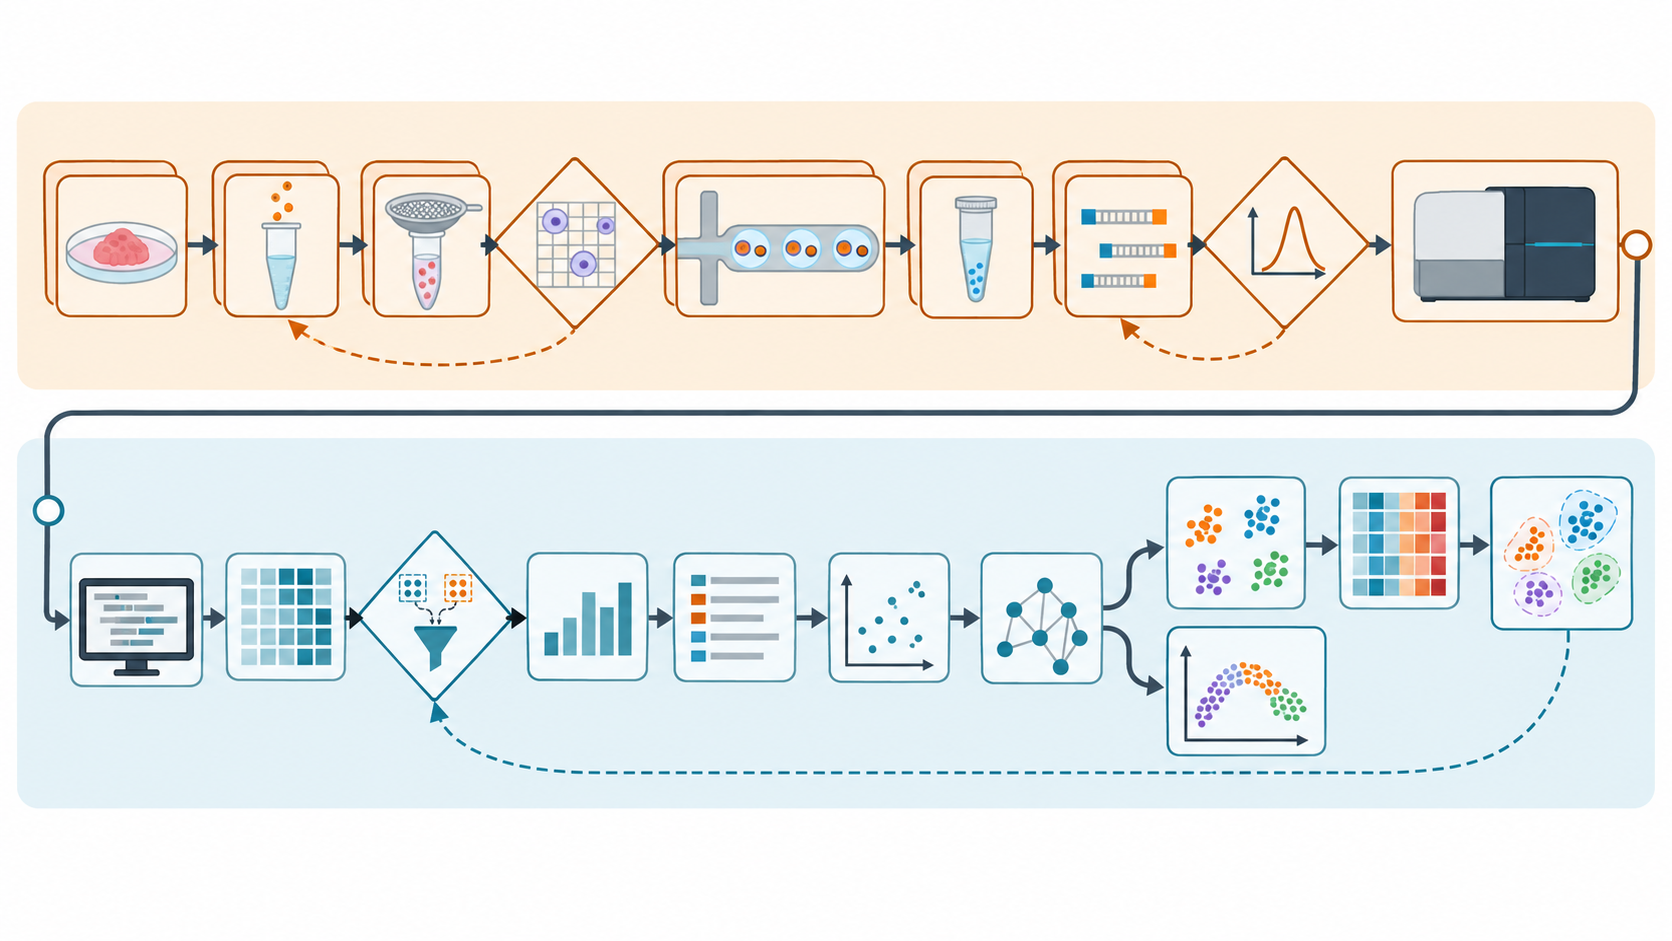
\includegraphics[width=\linewidth]{figures/ch06/ch06-05-v2-brief.png}};
\begin{scope}[x={(img.south east)},y={(img.north west)}]
  \tikzset{
    okmark/.style={draw=white,line width=0.6pt,fill=ChSixGood,text=white,circle,font=\sffamily\bfseries\tiny,inner sep=0.6pt,minimum size=3.6mm},
    ngmark/.style={draw=white,line width=0.6pt,fill=ChSixBad,text=white,circle,font=\sffamily\bfseries\tiny,inner sep=0.6pt,minimum size=3.6mm}
  }
  \node[okmark] at (0.07,0.85) {$\checkmark$};
  \node[okmark] at (0.16,0.85) {$\checkmark$};
  \node[okmark] at (0.25,0.85) {$\checkmark$};
  \node[ngmark] at (0.34,0.86) {$\times$};
  \node[okmark] at (0.25,0.60) {$\checkmark$};
  \node[okmark] at (0.46,0.85) {$\checkmark$};
  \node[okmark] at (0.58,0.85) {$\checkmark$};
  \node[okmark] at (0.67,0.85) {$\checkmark$};
  \node[ngmark] at (0.77,0.86) {$\times$};
  \node[okmark] at (0.72,0.61) {$\checkmark$};
  \node[ngmark] at (0.83,0.77) {$\times$};
  \node[ngmark] at (0.98,0.79) {$\times$};
  \node[okmark] at (0.08,0.44) {$\checkmark$};
  \node[okmark] at (0.17,0.44) {$\checkmark$};
  \node[ngmark] at (0.26,0.47) {$\times$};
  \node[ngmark] at (0.35,0.44) {$\times$};
  \node[okmark] at (0.44,0.44) {$\checkmark$};
  \node[okmark] at (0.53,0.44) {$\checkmark$};
  \node[okmark] at (0.62,0.44) {$\checkmark$};
  \node[okmark] at (0.68,0.42) {$\checkmark$};
  \node[okmark] at (0.68,0.25) {$\checkmark$};
  \node[okmark] at (0.84,0.52) {$\checkmark$};
  \node[ngmark] at (0.93,0.52) {$\times$};
  \node[okmark] at (0.58,0.14) {$\checkmark$};
\end{scope}
\end{tikzpicture}
\caption{按完整任务书整图生成的流程图底图（无文字）及逐项核对。绿色“$\checkmark$”为与步骤表一致的节点或箭头，红色“$\times$”为错误或缺失。本次生成虽然画对了近邻图分叉与三条指定反馈弧，但在质控菱形双样本叠卡、两处样本合并点、跨泳道连接箭头、可选小框位置及终点空白标签牌等 7 处位置仍存在结构偏差；因此终稿改为由作者绘制结构，模型只生成图标。}\label{fig:ch06-05}
\end{figure}

打印步骤表在图~\ref{fig:ch06-05} 上逐个节点、逐条箭头打勾核验，如实记录观察结果：本次生成确实做到了全图无文字，20 个主步骤图标的先后顺序、下排第 7 格近邻图向聚类与二维嵌入的分叉，以及三条指定虚线反馈弧（Q1 $\rightarrow$ W2、Q2 $\rightarrow$ W6、C11 $\rightarrow$ Q3）全部正确；但图上标出的 7 处红叉（$\times$）暴露出整图生成难以克服的结构短板：
\begin{enumerate}
\item \textbf{双样本叠卡不完整（上排第 4、第 8 格“$\times$”）：}提示词要求湿实验第 1 至 8 步每一步都画成双层叠放卡片，但模型只在 6 个圆角矩形步骤画了叠卡，两处菱形质控（Q1、Q2）却只画了单层菱形。
\item \textbf{两处样本合并点缺失（上排测序仪前与下排第 4 格“$\times$”）：}文库质控到测序仪之间只有单根箭头，没有画出两条样本文库线汇合入测序仪；下排第 4 格标准化柱状图处同样看不出两个样本的过滤后矩阵在此合并。
\item \textbf{跨泳道连接箭头不清（上排最右端“$\times$”）：}右上角连接圆圈直接贴在测序仪边框上，缺少从测序仪指向圆圈的独立交接箭头，也未留出放置产物 FASTQ 的位置。
\item \textbf{可选步骤位置错位（下排第 3 格“$\times$”）：}提示词要求把两个虚线可选小框（C3a、C3b）画在细胞质控菱形上方再汇入，模型却把两个带小点的虚线小方框直接塞进了菱形内部，无法叠加文字标签。
\item \textbf{终点与图标细节偏差（下排最右端“$\times$”）：}注释终点只画了包绕点簇的虚线轮廓，漏掉了提示词要求的空白圆角标签牌；上排第 6 步的 PCR 管画得偏长、像普通离心管，且部分器皿仍带渐变与立体透视。
\end{enumerate}

V2 实验证明：整图生成能提供色彩与风格方向，但逐项核对和返工的成本远高于直接画骨架，而且每次重生成都必须把全部二十多个节点和箭头从头复查一遍。

因此，更可靠的分工是改用\textbf{“图标表模式”（V3）}：不再让图像模型画箭头和泳道，而是在一张 $4 \times 3$ 网格的白底画布上，一次生成 12 个风格统一、彼此独立的步骤图标，切分后嵌入图~\ref{fig:ch06-03} 的确定性骨架。在 \scidraw{} 中，作者可从流程图入口（\sdtool{workflow-diagram-generator}）或科研绘图向导（\sdtool{figure-workflow}）“机制与流程图”路线进入绘图工作台（\sdtool{ai-drawing}），用提示词模式生成如下 12 宫格图标表：

\begin{Prompt}
A sheet of twelve flat vector scientific icons arranged in an even grid of four columns
and three rows on a pure white background. Each icon sits centred in its own invisible
square cell with wide white margins and does not touch any other icon. Uniform dark slate
outline of medium weight, flat fills, no gradients, no shadows, no 3D.
Row 1 (warm muted orange-brown accent #B5653A with pale beige fills):
 1. small piece of pink soft tissue on a shallow petri dish;
 2. conical centrifuge tube with three tiny droplets falling into it;
 3. round cell strainer mesh sitting on top of a tube;
 4. square counting grid with five round cells, one cell drawn darker.
Row 2 (same warm accent, except icon 8 in deep amber #8A6D1F):
 5. rectangular microfluidic chip with one channel pinching off round droplets,
    each droplet containing one small cell and one small bead;
 6. single small PCR tube with a closed cap;
 7. three short double-stranded DNA fragments, each with small coloured end caps;
 8. benchtop sequencing instrument: a box with a small slot holding a flow cell.
Row 3 (muted teal-blue accent #2F6F8F with pale blue-grey fills):
 9. computer monitor showing short horizontal bars aligned under one long bar;
10. square grid matrix of small cells with varied light-to-dark shading;
11. network of dots connected by thin edges;
12. four clusters of dots in different muted colours, with blank rounded tag shapes.
No text, no letters, no numbers, no labels, no arrows, no microscope, no DNA helix. 4:3.
\end{Prompt}

拿到 $4 \times 3$ 图标整表后，必须对 12 个图标逐格做科学核验：（1）浅培养皿上是粉红软组织小块，而非完整器官；（2）锥底离心管上方恰好落下 3 滴酶液，管上只有无字刻度线；（3）圆形筛网架在管口上；（4）计数方格内恰好 5 个圆细胞、1 个着色更深，无非圆杂物或文字；（5）微流控芯片单通道缩颈后方 3 个微滴，每滴含一较大细胞与一较小深色凝胶珠；（6）带扣盖的单个小 PCR 管；（7）3 段双链梯状短片段配彩色端帽，不是长链双螺旋装饰；（9）显示器内一条长横条下对齐多条短横条；（10）深浅变化的方格计数矩阵；（11）点与细边组成的近邻网络，无化学元素符号；（12）4 个不同色相的点簇，每簇旁各有一个空白圆角标签框。放大至 200\% 检查，全表无任何字母或数字残留。

唯独第 8 格（桌面测序仪）初稿不合格：机箱前方伸出了一个斜托盘，上面摆着条纹薄片，远看像一台办公打印机。由于图标表各格独立，我们无需重画全表，只需在 \scidraw{} 绘图历史中选中该测序仪图标作为参考图继续修改，下达只替换前方托盘为封闭式光学流动池卡匣的修改指令：

\begin{Prompt}
Edit only this one sequencing-instrument icon. Preserve its simple scientific icon style,
dark slate outline, white background, and square framing. Replace the printer-like front
paper tray and paper-output slot with a small closed optical flow-cell cartridge bay:
a glass rectangular microfluidic flow cell in a shallow enclosed cartridge, with tiny
parallel fluidic channels visible through a small window. Use flat pale beige fills with
a restrained deep amber #8A6D1F accent on the cartridge. No sheets of paper, no paper
trays, no keyboards, no text, no letters, no numbers, no labels, no logos. Aspect 1:1.
\end{Prompt}

单图标修改后，像打印机的外伸纸托消失，前面板中央换成了深琥珀色边框的玻璃微流控流动池窗口，内部可见平行折返流道。将图标表按 $4 \times 3$ 等分网格裁切、将近白背景转为透明通道并保留约 6\% 留白边距，即可放入骨架图。

\section{贯穿案例：单细胞 RNA 测序流程从初稿到终稿}

现在我们将小陈从 V1 初稿一路推进到 V4 终稿的完整过程串联起来：

\textbf{第一步：从 V1 初稿退回写步骤表与任务书。}
面对一句话提示词生成的 V1 初稿（图~\ref{fig:ch06-01}），小陈不再在提示词框里盲目打补丁，而是退回方法记录整理出表~\ref{tab:ch06-01} 的步骤表，并完成表~\ref{tab:ch06-02} 的九项实验条件核实。接着，她在 \scidraw{} 科研绘图向导（\sdtool{figure-workflow}）选择“机制与流程图”路线，替换默认任务书并下载本地副本：

\begin{Prompt}
【目的】让读者看清：从小鼠肺组织到细胞类型注释，每一步做什么、交给下一步什么；
         哪些是湿实验、哪些是计算；两个样本在哪里并行、在哪里合并；质控不通过时回到哪里。
【读者与用途】论文 Figure 1A 方法流程图；读者为熟悉分子生物学的同行。
         终稿可按双栏通栏 174 mm 宽缩排。
【必须出现的对象】步骤表 6-1 的全部主节点（W1–W6、Q1、Q2、S1、C1–C11）与可选节点
         （W3a、W3b、C3a、C3b、C6a），以及 6 类核心交接产物：单细胞悬液、带条形码的 cDNA、
         测序文库、FASTQ、过滤后计数矩阵、注释后的细胞图谱（另含原始矩阵与 UMAP 坐标）。
【关系与箭头含义】实线箭头 = 顺序与交接；虚线弧 = 反馈/返回；菱形 = 质控，两个出口；
         虚线框 = 可选步骤；圆形连接符 A = 跨行续接；流程箭头不表示因果。
【已知、假设与待确认】步骤顺序为通用流程，已确认；所有参数为〔作者填写〕，图中不写参数；
         整合/批次校正的位置为简化，图注说明。
【不可改变的科学信息】聚类与 UMAP 都从近邻图分出，UMAP 不连向聚类或注释；
         两个样本的文库在测序前混合，计数矩阵在标准化前合并。
【构图与标签】两条水平泳道：上为湿实验（含测序），下为计算分析，均从左到右阅读；
         上下由连接符 A（FASTQ）衔接。标签为中文，分子与软件名保留英文。
         湿实验暖色、计算冷色；每个泳道一种强调色。
【参考材料】步骤表 6-1；方法记录；Luecken & Theis 2019；Zheng et al. 2017。
【自查标准】节点数、箭头数、分支与合并点与步骤表逐一对应；没有未列出的步骤或装饰；
         图中无参数数值；在最终尺寸下 7 pt 文字可读。
\end{Prompt}

\textbf{第二步：用确定性骨架合并 AI 图标，合成 V4 终稿。}
在对比了确定性骨架（图~\ref{fig:ch06-03}）与 V2 整图生成（图~\ref{fig:ch06-05}）之后，小陈保持图~\ref{fig:ch06-03} 的全部节点坐标、箭头、分叉、反馈弧与文字标签一概不动，仅在 12 个主要步骤框正上方各放置一枚切分核验后的透明背景图标（01 $\rightarrow$ W1 组织采集；02 $\rightarrow$ W2 组织解离；03 $\rightarrow$ W3 过滤与清洗；04 $\rightarrow$ Q1 计数与活率；05 $\rightarrow$ W4 微滴捕获；06 $\rightarrow$ W5 逆转录与扩增；07 $\rightarrow$ W6 文库构建；08 $\rightarrow$ S1 混合与测序；09 $\rightarrow$ C1 比对与计数；10 $\rightarrow$ C2 细胞识别；11 $\rightarrow$ C7 $k$ 近邻图；12 $\rightarrow$ C11 细胞类型注释），其余节点保持纯文字框，避免过度装饰。合成后的终稿见图~\ref{fig:ch06-06}。

\begin{figure}[htbp]\centering
\resizebox{\linewidth}{!}{% FIG ch06-06 final (Chinese) — same structure as skeleton + icons%
\def\ChSixShowIcons{}%
% Shared styles for chapter 6 workflow TikZ figures.%
% Every figure inputs this file, so commands are defined with \providecommand.%
\providecolor{BookTeal}{HTML}{176C68}%
\providecolor{BookInk}{HTML}{23363E}%
\providecolor{BookRule}{HTML}{C8D6D6}%
\providecolor{BookPale}{HTML}{F1F6F5}%
\definecolor{WetPale}{HTML}{FBF1EA}%
\definecolor{Wet}{HTML}{B5653A}%
\definecolor{Seq}{HTML}{8A6D1F}%
\definecolor{DryPale}{HTML}{EEF4F7}%
\definecolor{Dry}{HTML}{2F6F8F}%
\definecolor{ChSixFeedback}{HTML}{7A8A90}%
\definecolor{ChSixBad}{HTML}{C0392B}%
\usetikzlibrary{arrows.meta,positioning,shapes.geometric,shapes.misc,fit,backgrounds,calc}%
\ifdefined\ChSixLayersReady\else%
  \pgfdeclarelayer{chsixlane}%
  \pgfsetlayers{chsixlane,background,main}%
  \def\ChSixLayersReady{}%
\fi%

\tikzset{%
  chsix/.style={font=\sffamily\scriptsize, text=BookInk, align=center},%
  flowstep/.style={%
    chsix, rounded corners=2pt, draw=Wet, line width=0.45pt, fill=white,%
    text width=19mm, minimum height=7.4mm, inner sep=1.3pt,%
  },%
  flowstepdry/.style={flowstep, draw=Dry},%
  flowstepseq/.style={flowstep, draw=Seq},%
  artifact/.style={%
    chsix, trapezium, trapezium left angle=70, trapezium right angle=110,%
    trapezium stretches=true,%
    draw=BookInk, line width=0.45pt, fill=white,%
    minimum height=6.2mm, inner sep=1.2pt,%
  },%
  gate/.style={%
    chsix, diamond, aspect=1.7, draw=BookInk, line width=0.45pt, fill=white,%
    text width=12mm, inner sep=0.6pt, minimum height=8mm,%
  },%
  opt/.style={flowstep, dashed, draw=BookInk!70},%
  optdry/.style={flowstepdry, dashed, draw=BookInk!70},%
  stack/.style={flowstep},%
  link/.style={-{Stealth[length=1.6mm]}, semithick, draw=BookInk},%
  linkthin/.style={-{Stealth[length=1.2mm]}, thin, draw=BookInk!80},%
  back/.style={-{Stealth[length=1.5mm]}, dashed, draw=ChSixFeedback},%
  conn/.style={%
    circle, draw=BookInk, line width=0.5pt, minimum size=4.6mm,%
    font=\sffamily\scriptsize\bfseries, inner sep=0pt, text=BookInk,%
  },%
  lanetitle/.style={font=\sffamily\bfseries\small, text=BookInk, align=left},%
  passlabel/.style={font=\sffamily\scriptsize, text=BookInk, fill=white, inner sep=0.7pt, align=center},%
  mergelabel/.style={font=\sffamily\scriptsize, text=BookInk, fill=white, inner sep=0.8pt, align=center},%
  taglab/.style={font=\sffamily\scriptsize, text=ChSixFeedback, fill=white, inner sep=0.8pt, align=center},%
  gramcap/.style={font=\sffamily\scriptsize, text=BookInk, align=left, anchor=west},%
}%

% Offset card behind a two-sample step. Text stays on the front node only.%
\providecommand{\ChSixCardBack}[1]{%
  \begin{pgfonlayer}{background}%
    \draw[Wet, line width=0.45pt, rounded corners=2pt, fill=white]%
      ([shift={(-0.55mm,0.55mm)}]#1.south west)%
      rectangle ([shift={(-0.55mm,0.55mm)}]#1.north east);%
  \end{pgfonlayer}%
}%
% #1 options, #2 name, #3 position (with parentheses), #4 text%
\providecommand{\ChSixCard}[4]{%
  \node[stack, #1] (#2) at #3 {#4};%
  \ChSixCardBack{#2}%
}%

\providecommand{\ChSixMaybeLabel}[1]{%
  \ifdefined\nolabels\else#1\fi%
}%

\providecommand{\ChSixIcon}[2]{%
  \ifdefined\ChSixShowIcons%
    \IfFileExists{#1}{%
      \node[anchor=south, inner sep=0] at ([yshift=0.7mm]#2.north)%
        {\includegraphics[height=5.4mm]{#1}};%
    }{}%
  \fi%
}%
%
% Chinese node labels for FIG ch06-03 / ch06-06%
\providecommand{\ChSixLaneWet}{湿实验与测序}%
\providecommand{\ChSixLaneDry}{计算分析}%
\providecommand{\ChSixTxtWone}{组织采集}%
\providecommand{\ChSixTxtWtwo}{组织解离}%
\providecommand{\ChSixTxtWthree}{过滤与清洗}%
\providecommand{\ChSixTxtWthreeA}{红细胞裂解}%
\providecommand{\ChSixTxtWthreeB}{死细胞去除}%
\providecommand{\ChSixTxtQone}{计数与\\活率}%
\providecommand{\ChSixTxtWfour}{微滴捕获与\\条形码标记}%
\providecommand{\ChSixTxtWfive}{逆转录与\\cDNA 扩增}%
\providecommand{\ChSixTxtWsix}{文库构建}%
\providecommand{\ChSixTxtQtwo}{文库\\质控}%
\providecommand{\ChSixTxtSone}{文库混合\\与测序}%
\providecommand{\ChSixTxtCone}{比对与\\UMI 计数}%
\providecommand{\ChSixTxtCtwo}{细胞识别}%
\providecommand{\ChSixTxtQthree}{细胞\\质控}%
\providecommand{\ChSixTxtCthreeA}{双细胞检测}%
\providecommand{\ChSixTxtCthreeB}{环境 RNA\\校正}%
\providecommand{\ChSixTxtCfour}{合并与\\标准化}%
\providecommand{\ChSixTxtCfive}{高变基因}%
\providecommand{\ChSixTxtCsix}{PCA 降维}%
\providecommand{\ChSixTxtCsixA}{整合（可选）}%
\providecommand{\ChSixTxtCseven}{k 近邻图}%
\providecommand{\ChSixTxtCeight}{聚类\\（Leiden）}%
\providecommand{\ChSixTxtCnine}{UMAP}%
\providecommand{\ChSixTxtCten}{标志基因}%
\providecommand{\ChSixTxtCeleven}{细胞类型\\注释}%
\providecommand{\ChSixArtSusp}{单细胞悬液}%
\providecommand{\ChSixArtCdna}{带条形码\\的 cDNA}%
\providecommand{\ChSixArtLib}{测序文库}%
\providecommand{\ChSixArtFastq}{FASTQ}%
\providecommand{\ChSixArtRaw}{原始计数\\矩阵}%
\providecommand{\ChSixArtFilt}{过滤后矩阵}%
\providecommand{\ChSixArtAtlas}{注释后的\\细胞图谱}%
\providecommand{\ChSixArtUmap}{UMAP 坐标\\（仅用于展示）}%
\providecommand{\ChSixQoneFail}{不合格：\\优化解离}%
\providecommand{\ChSixQtwoFail}{不合格}%
\providecommand{\ChSixCelevenFail}{发现低质量簇\\或分辨率不当}%
\providecommand{\ChSixMergeNote}{两样本在此合并}%
\providecommand{\ChSixPass}{通过}%
%
\begin{tikzpicture}[x=1cm,y=1cm]%
  % Row positions are set with relative anchors in ch06-workflow-draw.tex%
% so Chinese and English labels do not share one set of fixed centres.%
%
  % Workflow structure (FIG ch06-03 skeleton / ch06-06 final).%
% Requires ch06-styles and a label file. Nodes are placed from the node%
% above them so wrapped English labels cannot land on the next row.%
\coordinate (origin) at (0,0);%
% Final figures carry icons above the nodes; keep feedback arcs above them.%
\ifdefined\ChSixShowIcons
  \def\ChSixLift{6.6mm}%
  \def\ChSixArc{12.2mm}%
\else
  \def\ChSixLift{0mm}%
  \def\ChSixArc{8.4mm}%
\fi

% ----- Wet lab, row 1: collection through droplet capture -----%
\ChSixCard{anchor=north west}{nW1}{(origin)}{\ChSixMaybeLabel{\ChSixTxtWone}}%
\ChSixCard{anchor=west}{nW2}{([xshift=3.2mm]nW1.east)}{\ChSixMaybeLabel{\ChSixTxtWtwo}}%
\ChSixCard{anchor=west}{nW3}{([xshift=3.2mm]nW2.east)}{\ChSixMaybeLabel{\ChSixTxtWthree}}%
\node[gate, anchor=west] (nQ1) at ([xshift=3.6mm]nW3.east) {\ChSixMaybeLabel{\ChSixTxtQone}};%
\ChSixCard{anchor=west}{nW4}{([xshift=6.4mm]nQ1.east)}{\ChSixMaybeLabel{\ChSixTxtWfour}}%

\draw[link] (nW1) -- (nW2);%
\draw[link] (nW2) -- (nW3);%
\draw[link] (nW3) -- (nQ1);%
\draw[link] (nQ1) -- (nW4);%

\coordinate (arcQ1) at ($(nW2.north)!0.5!(nQ1.north)+(0,\ChSixArc)$);%
\draw[back] ([yshift=\ChSixLift]nQ1.north) -- ([yshift=\ChSixLift]nQ1.north |- arcQ1) -- ([yshift=\ChSixLift]nW2.north |- arcQ1) -- ([yshift=\ChSixLift]nW2.north);%
\node[taglab, anchor=south] (q1fail) at (arcQ1) {\ChSixMaybeLabel{\ChSixQoneFail}};%
\node[passlabel] (passQ1) at ($(nQ1.east)!0.5!(nW4.west)+(0,1.3mm)$) {\ChSixMaybeLabel{\ChSixPass}};%

\node[lanetitle, anchor=south west] (laneWet) at ([yshift=1.2mm]q1fail.north -| origin) {\ChSixMaybeLabel{\ChSixLaneWet}};%

% Optional lysis / dead-cell removal under filtering, product to their right.%
\node[opt, anchor=north] (nW3a) at ([yshift=-2.2mm]nW3.south) {\ChSixMaybeLabel{\ChSixTxtWthreeA}};%
\node[opt, anchor=north] (nW3b) at ([yshift=-1.8mm]nW3a.south) {\ChSixMaybeLabel{\ChSixTxtWthreeB}};%
\draw[linkthin] (nW3.south) -- (nW3a.north);%
\draw[linkthin] (nW3a.south) -- (nW3b.north);%
\node[artifact, anchor=north west] (aSusp) at ([xshift=3.2mm, yshift=-2.2mm]nW3.south east) {\ChSixMaybeLabel{\ChSixArtSusp}};%

% ----- Wet lab, row 2 (left-aligned; FASTQ is the hand-off into connector A) -----%
\ChSixCard{anchor=north west}{nW5}{([yshift=-10mm]nW3b.south -| nW1.west)}{\ChSixMaybeLabel{\ChSixTxtWfive}}%
\ChSixCard{anchor=west}{nW6}{([xshift=2.4mm]nW5.east)}{\ChSixMaybeLabel{\ChSixTxtWsix}}%
\node[gate, anchor=west] (nQ2) at ([xshift=2.4mm]nW6.east) {\ChSixMaybeLabel{\ChSixTxtQtwo}};%
\node[flowstepseq, anchor=west] (nS1) at ([xshift=6.2mm]nQ2.east) {\ChSixMaybeLabel{\ChSixTxtSone}};%
\node[artifact, anchor=west] (aFastq) at ([xshift=2.2mm]nS1.east) {\ChSixMaybeLabel{\ChSixArtFastq}};%
\node[conn, anchor=west] (nA) at ([xshift=2mm]aFastq.east) {A};%

\draw[link] (nW5) -- (nW6);%
\draw[link] (nW6) -- (nQ2);%
\draw[link] (nQ2) -- (nS1);%
\draw[link] (nS1) -- (aFastq);%
\draw[link] (aFastq) -- (nA);%
\node[passlabel] (passQ2) at ($(nQ2.east)!0.5!(nS1.west)+(0,1.3mm)$) {\ChSixMaybeLabel{\ChSixPass}};%

\coordinate (arcQ2) at ($(nW6.north)!0.5!(nQ2.north)+(0,\ChSixArc)$);%
\draw[back] ([yshift=\ChSixLift]nQ2.north) -- ([yshift=\ChSixLift]nQ2.north |- arcQ2) -- ([yshift=\ChSixLift]nW6.north |- arcQ2) -- ([yshift=\ChSixLift]nW6.north);%
\node[taglab, anchor=south] (q2fail) at (arcQ2) {\ChSixMaybeLabel{\ChSixQtwoFail}};%

\node[artifact, anchor=north] (aCdna) at ([yshift=-2mm]$(nW5.south)!0.5!(nW6.south)$) {\ChSixMaybeLabel{\ChSixArtCdna}};%
\node[artifact, anchor=north] (aLib) at ([yshift=-2mm]$(nW6.south)!0.5!(nQ2.south)$) {\ChSixMaybeLabel{\ChSixArtLib}};%

% ----- Computational lane -----%
\node[conn, anchor=north west] (nA2) at ([yshift=-7mm]aCdna.south -| origin) {A};%
\node[flowstepdry, anchor=west] (nC1) at ([xshift=3.2mm]nA2.east) {\ChSixMaybeLabel{\ChSixTxtCone}};%
\node[flowstepdry, anchor=west] (nC2) at ([xshift=3.6mm]nC1.east) {\ChSixMaybeLabel{\ChSixTxtCtwo}};%
\node[gate, anchor=west] (nQ3) at ([xshift=4.2mm]nC2.east) {\ChSixMaybeLabel{\ChSixTxtQthree}};%
\node[flowstepdry, anchor=west] (nC4) at ([xshift=4.2mm]nQ3.east) {\ChSixMaybeLabel{\ChSixTxtCfour}};%
\node[flowstepdry, anchor=west] (nC5) at ([xshift=3.6mm]nC4.east) {\ChSixMaybeLabel{\ChSixTxtCfive}};%

\draw[link] (nA2) -- (nC1);%
\draw[link] (nC1) -- (nC2);%
\draw[link] (nC2) -- (nQ3);%
\draw[link] (nQ3) -- (nC4);%
\draw[link] (nC4) -- (nC5);%

\node[mergelabel, anchor=south] (mergeNote) at ([yshift=1mm]nC4.north) {\ChSixMaybeLabel{\ChSixMergeNote}};%

\coordinate (arcDry) at ($(nC1.north)!0.5!(nQ3.north)+(0,\ChSixArc)$);%
\node[taglab, anchor=south, text width=28mm] (c11fail) at (arcDry) {\ChSixMaybeLabel{\ChSixCelevenFail}};%
\node[lanetitle, anchor=south west] (laneDry) at ([yshift=1.2mm]c11fail.north -| origin) {\ChSixMaybeLabel{\ChSixLaneDry}};%

% Optional doublet / ambient RNA under the cell-QC gate.%
\node[optdry, anchor=north east] (nC3a) at ([yshift=-2mm, xshift=-1mm]nQ3.south) {\ChSixMaybeLabel{\ChSixTxtCthreeA}};%
\node[optdry, anchor=north west] (nC3b) at ([yshift=-2mm, xshift=1mm]nQ3.south) {\ChSixMaybeLabel{\ChSixTxtCthreeB}};%
\draw[linkthin] (nQ3.south) -- (nC3a.north);%
\draw[linkthin] (nQ3.south) -- (nC3b.north);%
\draw[linkthin] (nC3a.south) -- ++(0,-2.4mm) -| (nC3b.south);%

\node[artifact, anchor=north] (aRaw) at ([yshift=-2mm]$(nC1.south)!0.5!(nC2.south)$) {\ChSixMaybeLabel{\ChSixArtRaw}};%
\node[artifact, anchor=north] (aFilt) at ([yshift=-2mm]nC4.south) {\ChSixMaybeLabel{\ChSixArtFilt}};%

% Fork: k-NN graph splits to clustering (continues) and UMAP (display only).%
\node[flowstepdry, anchor=north west] (nC6) at ([yshift=-4mm]aRaw.south -| nC1.west) {\ChSixMaybeLabel{\ChSixTxtCsix}};%
\node[flowstepdry, anchor=west] (nC7) at ([xshift=4mm]nC6.east) {\ChSixMaybeLabel{\ChSixTxtCseven}};%
\node[flowstepdry, anchor=west] (nC8) at ([xshift=5mm]nC7.east) {\ChSixMaybeLabel{\ChSixTxtCeight}};%
\node[flowstepdry, anchor=west] (nC10) at ([xshift=3.6mm]nC8.east) {\ChSixMaybeLabel{\ChSixTxtCten}};%
\node[flowstepdry, anchor=west] (nC11) at ([xshift=3.6mm]nC10.east) {\ChSixMaybeLabel{\ChSixTxtCeleven}};%
\node[optdry, anchor=north] (nC6a) at ([yshift=-2mm]nC6.south) {\ChSixMaybeLabel{\ChSixTxtCsixA}};%
\node[flowstepdry, anchor=north] (nC9) at ([yshift=-3.2mm]nC7.south) {\ChSixMaybeLabel{\ChSixTxtCnine}};%
\node[artifact, anchor=north, text width=22mm] (aUmap) at ([yshift=-1.8mm]nC9.south) {\ChSixMaybeLabel{\ChSixArtUmap}};%
\node[artifact, anchor=north] (aAtlas) at ([yshift=-2mm]$(nC10.south)!0.5!(nC11.south)$) {\ChSixMaybeLabel{\ChSixArtAtlas}};%

\draw[link] (nC5.south) -- ++(0,-2.5mm) -| (nC6.north);%
\draw[linkthin] (nC6.south) -- (nC6a.north);%
\draw[link] (nC6) -- (nC7);%
\draw[link] (nC7) -- (nC8);%
\draw[link] (nC8) -- (nC10);%
\draw[link] (nC10) -- (nC11);%
\draw[link] (nC7.south) -- (nC9.north);%

% Return from annotation to clustering, and the long return to cell QC.%
\coordinate (bus) at ([yshift=-4.5mm]aUmap.south);%
\draw[back] (nC11.south) -- (nC11.south |- bus) -- (nC8.south |- bus) -- (nC8.south);%
\draw[back] (nC11.east) -- ++(3.2mm,0) |- (c11fail.east);%
\draw[back] (c11fail.west) -| ([yshift=\ChSixLift]nQ3.north);%

% Connector A joins the lanes in the gutter between them.%
\draw[link] (nA.south) -- ++(0,-2.2mm) -| (nA2.north);%

\ChSixIcon{figures/ch06/icons/ch06-icon-01.png}{nW1}%
\ChSixIcon{figures/ch06/icons/ch06-icon-02.png}{nW2}%
\ChSixIcon{figures/ch06/icons/ch06-icon-03.png}{nW3}%
\ChSixIcon{figures/ch06/icons/ch06-icon-04.png}{nQ1}%
\ChSixIcon{figures/ch06/icons/ch06-icon-05.png}{nW4}%
\ChSixIcon{figures/ch06/icons/ch06-icon-06.png}{nW5}%
\ChSixIcon{figures/ch06/icons/ch06-icon-07.png}{nW6}%
\ChSixIcon{figures/ch06/icons/ch06-icon-08.png}{nS1}%
\ChSixIcon{figures/ch06/icons/ch06-icon-09.png}{nC1}%
\ChSixIcon{figures/ch06/icons/ch06-icon-10.png}{nC2}%
\ChSixIcon{figures/ch06/icons/ch06-icon-11.png}{nC7}%
\ChSixIcon{figures/ch06/icons/ch06-icon-12.png}{nC11}%

\begin{pgfonlayer}{chsixlane}%
  \node[rectangle, fit=(laneWet)(nW1)(nW4)(nW3b)(aSusp)(nA)(aCdna)(aLib)(q1fail),%
        fill=WetPale, draw=none, inner sep=1.1mm] {};%
  \node[rectangle, fit=(laneDry)(nA2)(nC5)(nC11)(nC6a)(aUmap)(aAtlas)(c11fail)(nC3a)(nC3b),%
        fill=DryPale, draw=none, inner sep=1.1mm] {};%
\end{pgfonlayer}%
%
\end{tikzpicture}%
}
\caption{液滴法单细胞 RNA 测序的实验与分析流程（示意）。上：湿实验与测序（暖色泳道）。对照与处理样本分别完成解离、捕获与文库构建（叠放的框），文库混合后测序。下：计算分析（冷色泳道），经连接符 A 由 FASTQ 衔接。菱形为质控，虚线弧表示不通过或结果异常时返回；虚线框为可选步骤。聚类与 UMAP 都基于主成分空间的 $k$ 近邻图，UMAP 仅用于展示。本图为通用流程的简化，未画出具体参数、细胞核测序、样本条形码复用、轨迹与差异丰度分析；整合/批次校正的位置因软件而异。图标由图像生成模型制作并经人工核对，流程结构与文字由作者绘制。}\label{fig:ch06-06}
\end{figure}

\textbf{第三步：编写双语图注并逐项填写终稿核验表。}
在 \scidraw{} 图注辅助（\sdtool{figure-legend}）起草的描述基础上，小陈补齐了简化范围、算法位置差异及 AI 分工声明，定稿中英文图注如下：

\begin{BookNote}
\textbf{图 6-6　液滴法单细胞 RNA 测序的实验与分析流程（示意）。} 上：湿实验与测序（暖色泳道）。对照与处理样本分别完成解离、捕获与文库构建（叠放的框），文库混合后测序。下：计算分析（冷色泳道），经连接符 A 由 FASTQ 衔接。菱形为质控，虚线弧表示不通过或结果异常时返回；虚线框为可选步骤。聚类与 UMAP 都基于主成分空间的 $k$ 近邻图，UMAP 仅用于展示。本图为通用流程的简化，未画出具体参数、细胞核测序、样本条形码复用、轨迹与差异丰度分析；整合/批次校正的位置因软件而异。图标由图像生成模型制作并经人工核对，流程结构与文字由作者绘制。

\medskip
\textbf{Figure 6-6 | Experimental and computational workflow for droplet-based single-cell RNA sequencing (schematic).} Top, wet-lab and sequencing steps (warm lane): control and treated samples are dissociated, captured and converted to libraries separately (stacked boxes) and pooled for sequencing. Bottom, computational analysis (cool lane), continued from FASTQ files via connector A. Diamonds are quality-control gates; dashed arcs return to an earlier step when a gate fails or results are anomalous; dashed boxes are optional steps. Clustering and UMAP are both computed from the $k$-nearest-neighbour graph in principal-component space; UMAP is used for display only. The diagram simplifies a generic protocol and omits parameters, single-nucleus protocols, sample multiplexing, trajectory and differential-abundance analyses; where integration sits varies between software packages. Icons were made with an image-generation model and checked by hand; the workflow structure and all text were drawn by the authors.
\end{BookNote}

交付前，小陈先用图片检查（\sdtool{figure-checker}）检查版面尺寸、灰度对比度与色觉可辨性，再对照表~\ref{tab:ch06-01} 逐行完成终稿核验记录（表~\ref{tab:ch06-04}）。

\begin{table}[htbp]\centering\footnotesize
\setlength{\tabcolsep}{4pt}
\renewcommand{\arraystretch}{1.15}
\caption{单细胞 RNA 测序流程图终稿（图~\ref{fig:ch06-06}）逐项核验记录。}\label{tab:ch06-04}
\begin{tabularx}{\linewidth}{@{}>{\raggedright\arraybackslash}p{22mm}YY@{}}
\toprule
\textbf{检查项} & \textbf{任务书与步骤表期望} & \textbf{图~\ref{fig:ch06-06} 终稿核验结果} \\
\midrule
节点数 & 主节点 20 个（湿实验与测序 W1–W6、Q1、Q2、S1 共 9 个；计算 C1–C11、Q3 共 11 个）+ 可选节点 5 个（W3a、W3b、C3a、C3b、C6a）+ 产物 8 个 & 全部在位，与图~\ref{fig:ch06-03} 骨架完全同构 \\
顺序箭头 & 每条实线箭头与表~\ref{tab:ch06-01}“下游”列一一对应 & 逐条核对一致，跨泳道由连接符 A 准确续接 \\
分叉关系 & C7 $\rightarrow$ C8（Leiden 聚类）、C7 $\rightarrow$ C9（UMAP）；Q3 下方 C3a $\parallel$ C3b & 分叉点与并行可选框连接正确 \\
样本合并 & S1（两个样本文库混合）；C4（两个样本过滤后矩阵合并） & W1–W6 双层叠卡至 S1 合并为单框；C4 上方标明合并 \\
反馈弧 & Q1 $\rightarrow$ W2；Q2 $\rightarrow$ W6；C11 $\rightarrow$ Q3；C11 $\rightarrow$ C8 & 四条虚线反馈弧线型、方向与文字说明全部正确 \\
质控出口 & Q1、Q2、Q3 各有正向通过与异常返回路径 & 菱形节点双出口齐全 \\
禁止关系 & C9 不连 C8、C11；无因果箭头；无未经确认的参数数值 & 已确认无错误连线、无参数数字 \\
图标与文字 & 12 个图标与主要步骤对应、200\% 放大无文字；软件与缩写保留英文；最终尺寸下节点文字 $\ge 6.5\text{ pt}$ & 12 个图标位置准确、无伪文字（测序仪图标需确认采用流动池卡匣修正版）；字号与可读性达标 \\
\bottomrule
\end{tabularx}
\end{table}

\section{AI 在这一步能做什么与不能做什么}

方法流程图各环节中 AI 与作者的职责边界汇总于表~\ref{tab:ch06-03}。

\begin{table}[htbp]\centering\footnotesize
\setlength{\tabcolsep}{3pt}
\renewcommand{\arraystretch}{1.15}
\caption{方法流程图制作中 AI 能做、不能做与作者要核对的内容。}\label{tab:ch06-03}
\begin{tabularx}{\linewidth}{@{}>{\raggedright\arraybackslash}p{18mm}YYY@{}}
\toprule
\textbf{环节} & \textbf{AI 能做} & \textbf{不能做 / 不应交给它} & \textbf{作者要核对} \\
\midrule
整理方法 & 从方法文字中抽出候选步骤，提示可能遗漏的产物、质控和分支 & 知道你实际做了哪些可选步骤；给出真实参数（它会补出“看起来合理”的数值） & 步骤表每一行与实验记录一致；所有参数来自记录，AI 补出的标为待确认 \\
结构 & 按描述生成“像流程图”的整图；草图模式参考上传的骨架布局 & 保证节点数、箭头方向、分支和合并点正确；草图不等于布局锁定 & 逐节点、逐箭头对照步骤表打勾 \\
图标与风格 & 生成风格一致的图标表；按指令修改单个图标；从历史图继续修改 & 保证图标在科学上准确（例如每滴一个细胞）；底图中写对术语 & 每个图标的科学含义；底图无文字 \\
文字 & —（本章终稿文字全部由 TikZ 写） & 图像模型中可靠拼写长术语 & 术语、缩写、软件名中英一致 \\
图注 & \sdtool{figure-legend} 根据图片起草描述 & 知道简化了什么、省略了什么、哪些参数待补 & 写明简化范围、可选步骤、图标来源与 AI 使用 \\
检查 & \sdtool{figure-checker} 检查尺寸、分辨率、灰度与色觉风险 & 判断流程在科学上是否正确 & 领域同行复核流程顺序 \\
\bottomrule
\end{tabularx}
\end{table}

\section{本章检查清单}

\begin{itemize}
\item 有一张步骤表，图中每个框都能在表中找到一行，表中每一行都在图中或在图注中声明省略。
\item 步骤（做什么）与产物（得到什么）分开画；关键交接处有产物。
\item 每个质控/判断有通过与不通过两个出口，不通过的去向与实验记录一致。
\item 并行处理画成并列，并标出合并点；可选步骤用统一的虚线样式，未做的步骤已删除。
\item 反馈/迭代用与顺序箭头不同的线型。
\item 湿实验与计算（或其他阶段）可一眼区分，颜色之外还有泳道标签。
\item 流程箭头只表示先后与交接；机制或因果信息写在注释或图注中。
\item 可视化步骤（如 UMAP）没有被画成分析步骤的上游。
\item 图中不出现未经确认的参数；底图无伪文字；所有文字可编辑。
\item 图注写明简化范围与图标的生成方式（本章示例图由图像模型生成，提示词与生成记录见本书仓库）。
\end{itemize}

\section{练习}

\begin{enumerate}
\item \textbf{改写方法记录：}选你自己论文方法部分的一段（或用第 6.2 节记录的前半段），整理成步骤表（ID、步骤、泳道、输入、产物、条件、质控、下游），并列出至少 5 项需要作者确认的条件。
\item \textbf{\scidraw{} 实操：}在科研绘图向导选“机制与流程图”路线，进入绘图，先用一句话生成你的流程图并保存为 V1；再写一份图标表提示词（不含文字，6–12 个图标）生成图标，选中历史图修改其中一个不合格的图标。在 PowerPoint、draw.io 或 TikZ 中按你的步骤表画骨架并放入图标。提交：V1、图标表、修改指令、终稿和逐项核对表。
\item \textbf{跨学科改错（计算机/数据科学）：}给出一张机器学习流程草图描述——“原始数据 $\rightarrow$ 特征标准化（用全部数据计算均值与方差）$\rightarrow$ 划分训练集/测试集 $\rightarrow$ 训练 $\rightarrow$ 在测试集评估”。指出流程中的数据泄漏（标准化参数应只由训练集计算，再应用到测试集），用本章语法重画为：先划分 $\rightarrow$ 训练集拟合标准化参数 $\rightarrow$ 同一参数分别变换训练集与测试集（并行分支）$\rightarrow$ 训练 $\rightarrow$ 评估，并写一句图注说明。
\end{enumerate}

\section*{参考文献}

\begin{itemize}
\item Heumos L, Schaar AC, Lance C, Litinetskaya A, Drost F, Zappia L, Lücken MD, Strobl DC, Henao J, Curion F, Single-cell Best Practices Consortium, Schiller HB, Theis FJ. Best practices for single-cell analysis across modalities. \textit{Nature Reviews Genetics}. 2023;24:550--572. doi:10.1038/s41576-023-00586-w
\item Hwang B, Lee JH, Bang D. Single-cell RNA sequencing technologies and bioinformatics pipelines. \textit{Experimental \& Molecular Medicine}. 2018;50:96. doi:10.1038/s12276-018-0071-8
\item Islam S, Zeisel A, Joost S, La Manno G, Zajac P, Kasper M, Lönnerberg P, Linnarsson S. Quantitative single-cell RNA-seq with unique molecular identifiers. \textit{Nature Methods}. 2014;11(2):163--166. doi:10.1038/nmeth.2772
\item Luecken MD, Theis FJ. Current best practices in single-cell RNA-seq analysis: a tutorial. \textit{Molecular Systems Biology}. 2019;15(6):e8746. doi:10.15252/msb.20188746
\item Macosko EZ, Basu A, Satija R, Nemesh J, Shekhar K, Goldman M, Tirosh I, Bialas AR, Kamitaki N, Martersteck EM, Trombetta JJ, Weitz DA, Sanes JR, Shalek AK, Regev A, McCarroll SA. Highly parallel genome-wide expression profiling of individual cells using nanoliter droplets. \textit{Cell}. 2015;161(5):1202--1214. doi:10.1016/j.cell.2015.05.002
\item Traag VA, Waltman L, van Eck NJ. From Louvain to Leiden: guaranteeing well-connected communities. \textit{Scientific Reports}. 2019;9:5233. doi:10.1038/s41598-019-41695-z
\item van den Brink SC, Sage F, Vértesy Á, Spanjaard B, Peterson-Maduro J, Baron CS, Robin C, van Oudenaarden A. Single-cell sequencing reveals dissociation-induced gene expression in tissue subpopulations. \textit{Nature Methods}. 2017;14:935--936. doi:10.1038/nmeth.4437
\item Wolf FA, Angerer P, Theis FJ. SCANPY: large-scale single-cell gene expression data analysis. \textit{Genome Biology}. 2018;19:15. doi:10.1186/s13059-017-1382-0
\item Wolock SL, Lopez R, Klein AM. Scrublet: computational identification of cell doublets in single-cell transcriptomic data. \textit{Cell Systems}. 2019;8(4):281--291.e9. doi:10.1016/j.cels.2018.11.005
\item Wong B. Points of view: Gestalt principles (Part 2). \textit{Nature Methods}. 2010;7:941. doi:10.1038/nmeth1210-941
\item Wong B. Points of view: simplify to clarify. \textit{Nature Methods}. 2011a;8:611. doi:10.1038/nmeth.1660
\item Wong B. Points of view: arrows. \textit{Nature Methods}. 2011b;8:701. doi:10.1038/nmeth.1676
\item Young MD, Behjati S. SoupX removes ambient RNA contamination from droplet-based single-cell RNA sequencing data. \textit{GigaScience}. 2020;9(12):giaa151. doi:10.1093/gigascience/giaa151
\item Zheng GXY, Terry JM, Belgrader P, Ryvkin P, Bent ZW, Wilson R, Ziraldo SB, Wheeler TD, McDermott GP, Zhu J, Gregory MT, Shuga J, Montesclaros L, Underwood JG, Masquelier DA, Nishimura SY, Schnall-Levin M, Wyatt PW, Hindson CM, Bharadwaj R, Wong A, Ness KD, Beppu LW, Deeg HJ, McFarland C, Loeb KR, Valente WJ, Ericson NG, Stevens EA, Radich JP, Mikkelsen TS, Hindson BJ, Bielas JH. Massively parallel digital transcriptional profiling of single cells. \textit{Nature Communications}. 2017;8:14049. doi:10.1038/ncomms14049
\end{itemize}

% TODO: figures/ch06/ch06-05-v2-scidraw.png (SciDraw AI screenshot for optional panel B of FIG ch06-05, not present on disk)
% TODO: figures/ch06/ch06-workflow-draw.tex line 119 references figures/ch06/icons/ch06-icon-08.png instead of figures/ch06/icons/ch06-icon-08-corrected.png
